An updated and more complete version of this chapter can be found in \cite{Ardhuin&al.2019}. 
The generation and propagation of microbaroms, which are atmospheric acoustic waves, will be treated in a chapter \ref{chbaroms}.

\section{A short history of microseism observations}
In the early days of seismology in the late 19th century, a background 
noise of varying amplitude was detected. \cite{Bertelli1872} performed measurements in Italy and  found that the amplitude of these microseisms changed 
with the passing of storms. By the year 1900, the phenomenon was measured all around the globe, and \cite{Algue1900} related measurements in the Philippines to the passage of Typhoons.  Many observations 
followed and the investigation of microseisms has grown to been a big branch of seismology. What was a curiosity is now an important source of data for studying the Earth's structure as microseisms provide a continuous source of signals that can be used to infer properties of the solid Earth \citep{Shapiro&al.2005} or to investigate the ocean wave climate \citep{Zopf&al.1976} because, yes, microseisms are generated by 
ocean waves, we will see how this happens. 

 All seismometer measurements on Earth contain microseisms. These seismic waves propagate through 
the solid Earth and oceans, with a displacement amplitude that rarely exceeds 10 microns, 
and a dominant wave period typically between 3 and 10~s.
%%%%%%%%%%%%%%%%%%%%%%%%%%%%%%%%%%%%%%%%%%%%%%%%%%%%%%%%%%%%%%%%%%%%%%%%%%%%%
\begin{figure}[htb]
\centerline{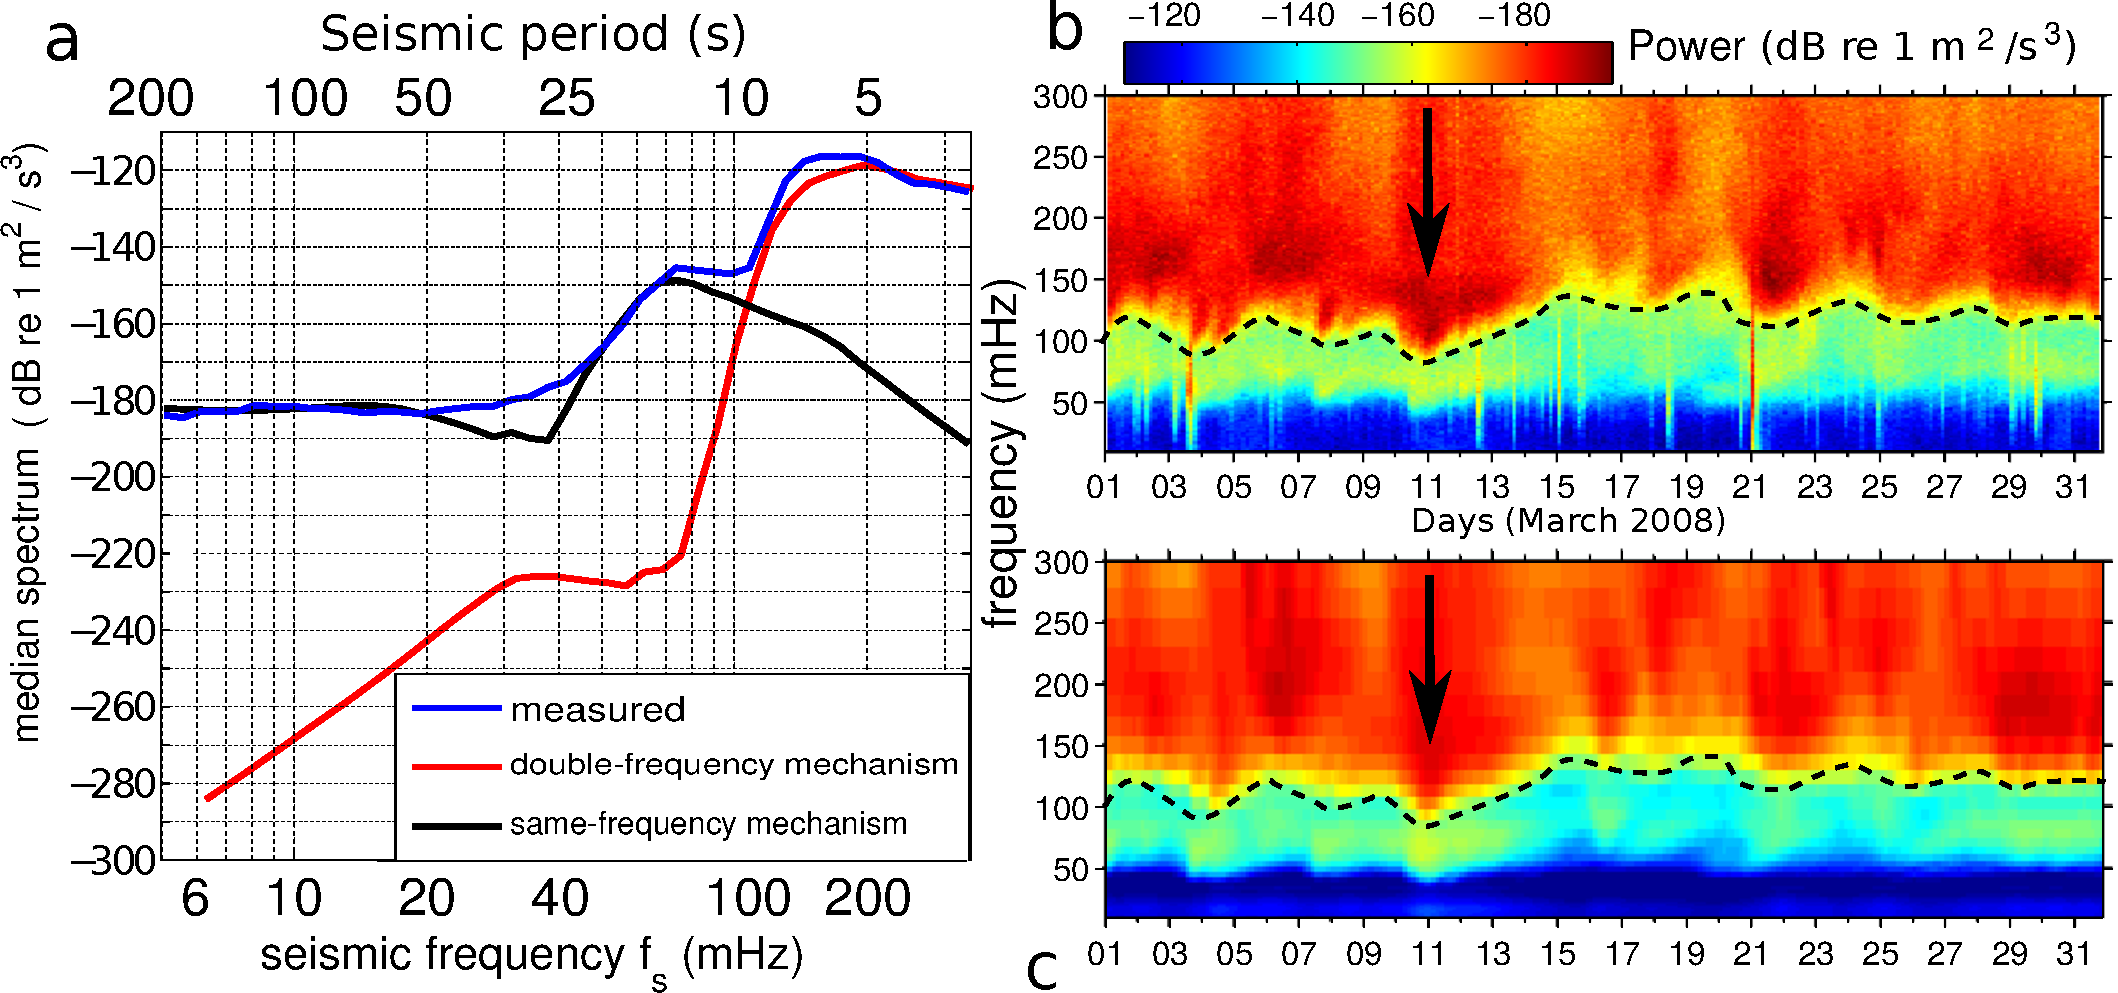
\includegraphics[width=\textwidth]{FIGS_CH_SISMO/microseisms_spectra_small.pdf}}
%\vspace{3.64in}
  \caption{Measured and modeled seismic spectra. (a) Median vertical acceleration power spectra in March 2008 at the French SSB seismic station, 
  located near Saint-Etienne, France. (b) observed and (c) modeled spectra in March 2008 following \cite{Ardhuin&al.2015}. 
  Light blue to red vertical stripes correspond to earthquakes (not modeled).   Contrary to intuition, the direct impact of waves 
  at the shoreline shown on these pictures is not the main source of the microseisms recorded at remote stations. Instead,
  seismic waves are mostly generated by two mechanisms: a same-frequency mechanism involves wave propagation over varying topography in intermediate 
  water depth, and a double-frequency mechanism that involves the interaction of waves in opposite directions. 
  The dashed line separates the low frequencies where the same-frequency mechanism dominates from the higher frequencies explained by the 
  double-frequency mechanism. The Johanna storm, marked by the vertical arrow on March 10, is conspicuous with powerful and low frequency microseisms. %  Pictured right: coastal impact of Johanna at G{\^a}vres and Le Conquet, France. 
}
\label{fig:microseism_spectra}
\end{figure}
%%%%%%%%%%%%%%%%%%%%%%%%%%%%%%%%%%%%%%%%%%%%%%%%%%%%%%%%%%%%%%%%%%%%%%%%%%%%%

From seismograph records, the apparently random signal gives a power spectrum with very robust features. \cite{Stutzmann&al.2000} showed how the 
noise level generally decreases from island stations to stations deep inside continents, with a classical shape. When the 
vertical acceleration is considered, the noise generally has 2 broad peaks.  The so-called `secondary' peak lies at periods between 
3 and 10~s, typically half of the dominant ocean wave periods, and it is the most energetic. The weaker 'primary' peak has the same period as typical swells, between 10 and 25 s, and 
a broad interval of noise is found at periods above 30~s. That long period range is called the hum. 

In all of these frequency bands, the seismic waves can be separated in different modes, 
\begin{itemize}
\item Raleigh waves: these are waves that follow the surface of the crust, with a motion in the plane of propagation, and an exponential decrease of the 
motion amplitude towards the center of the  Earth. Within 2000~km from the source, these Rayleigh waves usually dominate the microseisms recorded in the 3 to 10~s period band. 
\item Love waves: these are waves that follow the surface of the crust, with a motion out of the plane of propagation, and an exponential decrease of the 
motion amplitude towards the center of the  Earth. 
\item compressive body (P) waves: these waves travel through the Earth mantle, with a motion in the direction of propagation. 
\item shear body (S) waves: these waves travel through the Earth mantle, with a motion transverse to the direction of propagation, either in the vertical direction,
these are then called SV waves, or horizontal direction, and they are called SH waves.
\end{itemize}

Ongoing efforts are now explaining how and where this noise comes from, which may have 
some important application for seismology or the study of the ocean wave climate. The acoustic noise field in the ocean is also part of 
this seismic noise field, with some wave modes that have important signatures in the water column and in the atmosphere.

A key feature of the generation of microseisms is that it transfers energy 
from ocean waves that are slow, with typical phase speeds of  10~m/s, to the much faster seismic waves with speeds of several km/s. 
How can slow waves excite fast waves? 

\section{The particular case of standing ocean waves}
\cite{Miche1944b} was the first to show that, at second order in the wave steepness, the pressure under stationary waves oscillates in time but does not decay with depth. Clearly, 
we cannot generally assume that $C(t)$ in the Bernoulli equation is zero.  
Taking two propagating waves that give standing waves, with elevations $a \cos(kx - \sigma t)$ and $a \cos(kx + \sigma t)$, going in directions towards  $x>0$ and $x<0$. Their sum is 
the stationary wave,
\begin{eqnarray}
 \zeta &=& 2 a \cos(kx) \cos (\sigma t).\\
 w &=& - 2 a \sigma \frac{\sinh(kz + kD)}{\sinh(kD)} \cos(kx) \sin (\sigma t).\\
\end{eqnarray}

It is particulary interesting to look at the horizontally averaged pressure at depth $z$ using eq. 
(10.30)  %\ref{p_z}
\begin{equation}
\overline{p}(z)= \rho_w g (\zeta -z) + \rho_w \frac{\partial }{\partial t}\overline{\zeta w(\zeta)} -\rho_w \overline{w(z)^2}.
\end{equation}
The last two terms are deviations from the hydrostatic pressure and they give the non-hydrostatic (NH) pressure,  
\begin{equation}
\overline{p}_{\mathrm{NH}}(z)=-2 \rho_w  a^2 \sigma^2 \left[   \cos(2 \sigma t)  + \frac{\sinh^2(kz+kD)}{\sinh^2(kD)}  \sin^2(\sigma t)   \right].\label{sismo:p_NH}
\end{equation}
While the second term does not oscillate in time and decays with depth, the first term 
oscillates at a period equal to half of the propagating wave period, but is uniform over the vertical. 
%%%%%%%%%%%%%%%%%%%%%%%%%%%%%%%%%%%%%%%%%%%%%%%%%%%%%%%%%%%%%%%%%%%%%%%%%%%%%
\begin{figure}
\centerline{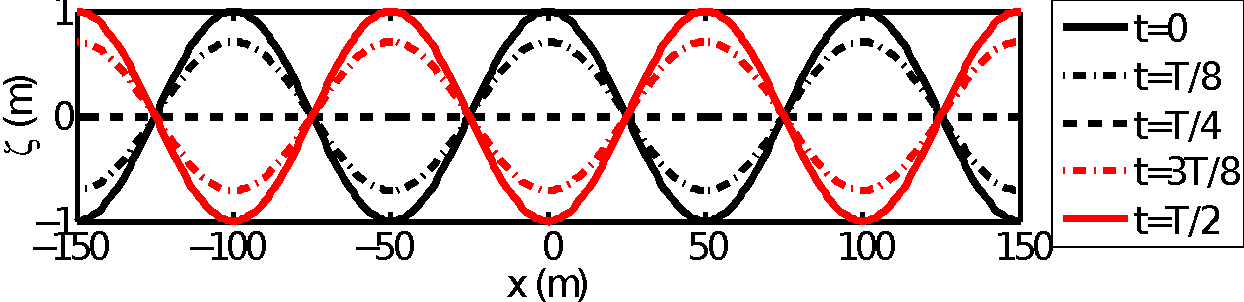
\includegraphics[width=\textwidth]{FIGS_CH_SISMO/standing_wave.pdf}}
%\vspace{3.64in}
  \caption{Schematic positions of the free surface in a stationary wave at different phases of the period $T$ of the progressive wave.}
\label{fig:standing}
\end{figure}
%%%%%%%%%%%%%%%%%%%%%%%%%%%%%%%%%%%%%%%%%%%%%%%%%%%%%%%%%%%%%%%%%%%%%%%%%%%%%

This fluctating pressure, predicted by \cite{Miche1944b}, was interpreted by \cite{Longuet-Higgins1950} as the vertical force that is necessary 
to compensate the fluctuations of the vertical momentum per unit surface 
\begin{equation}
M_z=\overline{\int_{-h}^{\zeta}\rho_w w {\mathrm d}z} \simeq \rho_w \overline{\zeta w(\zeta)}.
\end{equation}
This momentum is only non-zero when  $w$ and $\zeta$ are correlated, and at depth $d M_z /dt = p_{\mathrm{NH}} (z \rightarrow \infty)$. 

It should be noted, also, that the first term in pressure $\overline{p}_{\mathrm{NH}}$ is lowest when the wave amplitude is maximum, contrary to the second term. 
In the limit of shallow water $kD \ll 1$ and we have $\overline{p}_{\mathrm{NH}}(z) = 0$.  

Of course, the surface pressure is not immediately transmitted at large depth, and a more detailed description 
requires to take into account the compressibility of sea water. In reality, the surface oscillations produce acoustic 
waves that radiate in the water column \citep{Longuet-Higgins1950}, and are easily recorded at the ocean bottom \citep{Farrell&Munk2008}. 
Eq. (\ref{sismo:p_NH}) was verified in the laboratory by  \cite{Cooper&Longuet-Higgins1951}. 

Compared to the classical studies of ocean waves, the investigation of seismic and acoustic noise requires to relax two of the hypothesis made in chapter 2. Namely, 
we will have to take into accound the compressibility of sea water and air, and we will also need to allow the sea bottom to deform under the varying water pressure. 

In the case of exactly standing waves, the associated acoustic waves is propagating along the vertical. So this is not yet giving the seismic Rayleigh waves observed on land as surface waves. But the ocean waves are not monochromatic, so that it is much more likely to have interactions of waves with different wavenumbers rather than waves  with exactly opposing direction and frequency.  In fact, mathematically, the weight of these exactly opposing waves is zero. We thus need to generalize the standing wave to what we will find to be supersonic wave groups in the next section. 


\section{Wave-wave interaction theory for microseism generation}
Here we generally follow the method of \cite{Hasselmann1963c} with several corrections exposed by \cite{Ardhuin&Herbers2013}. 
In this process we also compute properties of Rayleigh waves in the presence of a water layer, which was first done by 
\cite{Stoneley1926}, and is covered in seismology textbooks such as \cite{Lay&Wallace1995},page 133, note the typo with  $\rho_w$ and $\rho_s$ exchanged in the dispersion relation.



\subsection{Wavenumber diagrams and isotropy of microseism sources}
We have seen in the previous chapters that wave components of frequency $f$ and wavenumber vector $\kb$ can 
interact with another wave or a change in medium (water depth or current) that has a frequency $f'$ and wavenumber $\kpb$, giving rise 
to a wave of frequency $f_s=f+f'$ and wavenumber $\Kb=\kb+\kpb$. The general theory of such interactions was sumarized by \cite{Hasselmann1966}. %and exposed in chapter \ref{chwwscat}. 

If the phase speed $2 \pi (f+f')/|\kb+\kpb|$ matches the speed of a seismic mode, 
then there is a resonance and interaction of waves with that seismic mode. In the case of microseisms, the ocean waves transfer energy to the seismic wave. 
Conversely, the vertical shaking of water, usually in the laboratory, gives rise to standing waves in the water, also known as Faraday waves. 

For seismic frequencies $f_s$ around $0.2$~Hz, the phase speed of seismic waves is larger 1.5~km/s, such large speed can only be achieved if $K << k$, which imposes $\kpb \simeq - \kb$, as illustrated on 
figure \ref{fig:kpluskprime}. The two neear-resonant configurations produce seismic waves that travel in very different directions. However, compared to that 
of the ocean waves, a 1\% change in the wave vector $\kb$ is generally negligible, because the half-width of the wave spectrum in frequency and direction is generally of the order of 5\% or more, 
and the wave energy spectral density $E(f,\theta)$ is the same if $\kb$ changes by only 1\%. Hence, 
at the spectral peak, the source of microseisms is isotropic. 
%%%%%%%%%%%%%%%%%%%%%%%%%%%%%%%%%%%%%%%%%%%%%%%%%%%%%%%%%%%%%%%%%%%%%%%%%%%%%
\begin{figure}[htb]
\centerline{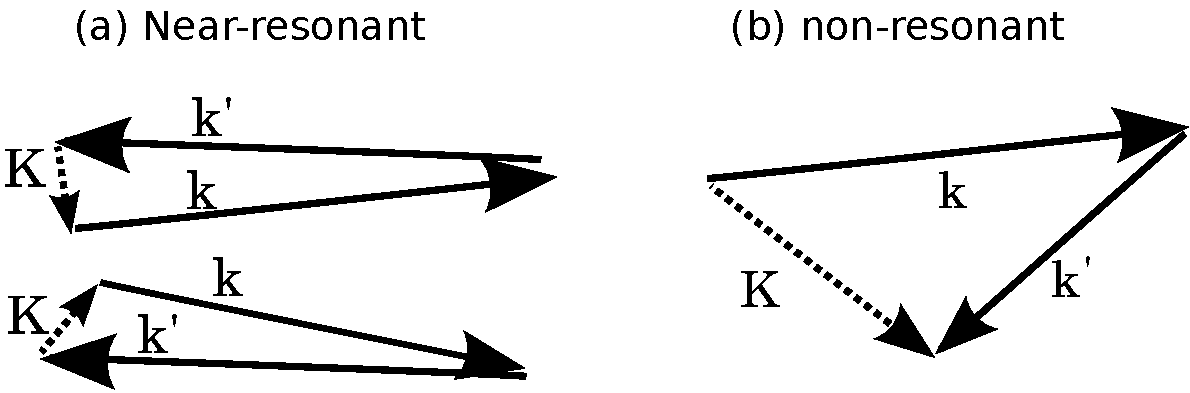
\includegraphics[width=\textwidth]{FIGS_CH_SISMO/Fdiagram3.pdf}}
%\vspace{3.64in}
  \caption{Typical configuration of interacting wave components}
\label{fig:kpluskprime}
\end{figure}
%%%%%%%%%%%%%%%%%%%%%%%%%%%%%%%%%%%%%%%%%%%%%%%%%%%%%%%%%%%%%%%%%%%%%%%%%%%%%

We can distinghish two mechanisms that give rise to these interactions, 
\begin{itemize}
 \item A same-frequency mechanism:  $\kpb$ corresponds to a change in depth or current, this is usually fixed in time or at least much slower than the waves, hence $f'=0$ and $f_s=f$, the seismic 
 waves have the same frequency as the ocean waves. 
 \item A double-frequency mechanism:  $\kpb$ corresponds to another wave component. Since  $\kpb \simeq - \kb$, we also have   $|\kpb| \simeq |\kb|$  and $f \simeq f'$, thus $f_s \simeq 2 f$: the 
 microseism have a frequency that is the double of the ocean wave frequency. 
\end{itemize}

Figure \ref{fig:microseism_spectra} shows that the same-frequency mechanism only  explains the hum and primary microseism, while the double-frequency mechanism explains the 
higher frequency secondary peak.  We will now give more theoretical details for each mechanism.


\subsection{Motion in the water and equivalent wave-induced pressure}
We follow here the theory of \cite{Hasselmann1963c} made for waves in deep water ($kD >> 1$), including the correction by \cite{Ardhuin&Herbers2013} for  finite water depth. We also note that a more detailed description is detailed for the case of the atmospheric pressure in chapter \ref{chbaroms} about microbaroms. 

From \cite{Longuet-Higgins1950}, we know that at first order the wave motion is given by Airy theory as exposed in chapter 2. 
At second order, the motion is forced at the surface by the interaction of pairs of linear (first order) solutions. This is thus the exact same problem that is solved in chapter \ref{ch_nonlin}, 
with the only change caused by compressibility. 

We decompose the water density into a mean value
$\rho_w$ and a perturbation $\rho \ll \rho_w$. 
Neglecting stratification effects due to temperature and salinity, 
the fluctuations in pressure $p$ and water density $\rho$ are related by an equation of state, 
which involves the speed of sound in water $\alpha_w$ \citep[][eq. 32]{Lighthill1978}.
\begin{eqnarray}
  \frac{d p}{d t}= \alpha_w^2 \frac{d \rho}{d t} \label{eq:state},
\end{eqnarray}

We still assume that the motion is irrotational so that the velocity field is still given by the gradient of 
the velocity potential $\phi$.  
The conservation of mass of sea water is 
\begin{eqnarray}
\frac{d \rho}{d t}&=& - \rho_w \nabla^2 \phi - \rho_w \frac{\partial^2 \phi}{\partial z^2}  \label{eq:sismo_rho_w}.
\end{eqnarray}


Equations (\ref{eq:sismo_rho_w})--(\ref{eq:state}) can be combined to eliminate $\rho$, 
\begin{eqnarray}
\frac{d p}{d t}=   -\rho_w \alpha_w^2 \left[ 
\nabla^2 + \frac{\partial^2 }{\partial z^2}\right] \phi \label{eq:sismo_p_w2a}
\end{eqnarray}

From eq. (\ref{eq:state}), the water density is only a function of the pressure. 
The two unknowns $p$ and $\phi$ are also related by the momentum conservation equation, 
with can be cast in the form of Bernoulli's equation 
 \citep[see e.g.][section 20]{Lamb1932},
\begin{equation}
    \frac{\partial \phi}{\partial t} = 
    -\frac{1}{2}\left[
    \left|\bnabla \phi\right|^2
    +\left(\frac{\partial \phi}{\partial z}\right)^2
    \right]-\frac{p}{\rho_w} - gz + C(t),
\label{Bernoulli2}
\end{equation}
with $C(t)$ a time-varying but spatially uniform function.

Therefore, instead of our usual Laplace equation we now have this acoustic wave equation in the body of the fluid 
\citep{Brekhovskikh&al.1973}, 
\begin{equation}
    \frac{\partial^2 \phi}{\partial t^2}  -\alpha_w^2 
\nabla_3^2  \phi    =  - \frac{\partial}{\partial t} (\nabla_3 \phi)^2 - g \frac{\partial \phi}{\partial z}. 
\label{eq:wavessimple}
\end{equation}
Where $\nabla_3$ is the 3-component nabla operator. If you remember chapter 2, this is the equation that will give us the vertical structure of the wave field, which is now an acoustic wave field. 

Now, in the case of microseisms, \cite{Longuet-Higgins1950} has shown that the non-linear forcing terms in the acoustic wave equation (\ref{eq:wavessimple}) produce negligible terms when $\sigma\simeq 0.5$~s$^{-1}$, so that we can use 
the linearized acoustic wave equation for the second order velocity potential $\phi_2$, 
\begin{equation}
\left[\frac{\partial^2 }{\partial t^2}  + \alpha_w^2 \left(
\nabla^2 + \frac{\partial^2 }{\partial z^2} - \frac{g}{\alpha_w^2} \frac{\partial }{\partial z} \right) \right]\phi_2   = 0 \quad {\mathrm for} \quad -h \leq z \leq 0. \label{eq:acoustic_linear}
\end{equation}
But if you really want to know more about the effect of these extra terms, do not worry, they cannot be neglected in the atmosphere when we consider microbaroms in chapter \ref{chbaroms}. 

With these approximations, The link between the ocean waves and the acoustic waves only comes from the  boundary conditions. As noted by \cite{Hasselmann1963c}, in the surface boundary condition, the interaction of first order wave motion is equivalent to a surface pressure $\widehat{p}_2$ given by eq. (\ref{eq:p2surf}). 
We note that this is not the true atmospheric pressure, for that you can go to  chapter \ref{chbaroms}, but the pressure that is goes into the surface boundary condition for $\phi_2$ and that makes it equivalent to a situation with a flat sea surface with  $\widehat{p}_2$ imposed on the surface. 
We note that the last term of eq. (\ref{eq:p2surf}) was  absent in \cite{Hasselmann1963c}  because he only considered waves in deep water where $kD  \gg 1$. As a result, that is also missing in  \cite{Webb2007} and was corrected by \cite{Ardhuin&Herbers2013}. These authors also found a source of acoustic energy in the bottom boundary condition.

Using (\ref{eq:p2surf}) the spectrum of the equivalent surface pressure can be expressed in terms of quadratic products of the (linear) sea surface elevation spectrum   
\begin{equation}
E(k_x,k_y)  = 2 \lim_{\left|d \kb \right| \ttz } \frac{\left|Z_{1,\kb}^{+}\right|^2}{\mathrm{d}k_x \mathrm{d}k_y}
\end{equation}
with a coupling coefficient given by eq. (\ref{Dz}) that simplifies for $K \simeq 0$ to   
\begin{equation}
   D_z\left(\kb,1,-\kb,1\right)   =  - 2 \sigma^2\left[1 + \frac{1}{4 \sinh^2(kh)}\right]. \label{Dz_keq0}
\end{equation}

For any value of $kD$, 
the coupling coefficient given by eq. (\ref{Dz_keq0}) differs from the full second order coefficient for the bottom pressure
\citep[e.g. eq. 4 in][]{Herbers&Guza1991}, 
which also involves the Bernoulli head (the bracket in eq. \ref{Bernoulli2}). However, that extra term 
is also relevant to the generation of seismic noise due to the  
bottom boundary condition that couples the solid crust to the water column. Indeed, the second-order 
pressure perturbation at the bottom writes, 
\begin{equation}
p_2(-h)=- \rho_w \frac{\partial \phi_2}{\partial t} + \widehat{p}_{2,\mathrm{bot}}, \label{pb}
\end{equation}
where the Bernoulli head contribution to the pressure can be expressed from the first order wave amplitudes, 
\begin{equation}
\widehat{p}_{2,\mathrm{bot}}= \rho_w \sum_{\kb,s,\kpb,s'}  D_{pb} \left(\kb,s,\kpb,s',z=-h\right) Z_{1,\kb}^{s} Z_{1,\kpb}^{s'} 
 \mathrm{e}^{\mathrm{i}
     \Theta(\kb,\kpb,s,s')}\label{P2bot},
\end{equation}
with a coupling coefficient $D_{pb}$ given by eq. (\ref{Dpb}).

We may interpret the bottom pressure (\ref{pb}) as the sum of the surface forcing $\widehat{p}_{2,\mathrm{surf}}$ transmitted 
to the bottom by  $\phi_2$, and  a direct effect of the Bernoulli head at the bottom which 
is an additional forcing $\widehat{p}_{2,\mathrm{bot}}$ that partly cancels $\widehat{p}_{2,\mathrm{surf}}$. 

We shall see in the next section that the forcing term for seismic noise 
is $\widehat{p}_{2,\mathrm{surf}} +\cos(lh) \widehat{p}_{2,\mathrm{bot}}$, with $l \leq K \ll k$ 
the vertical wavenumber in the water.  For shallow water gravity waves, $kh \ll 1$ and thus $\cos(lh) \simeq 1$ so that 
the effective forcing term becomes $\widehat{p}_{2,\mathrm{surf}} + \widehat{p}_{2,\mathrm{bot}}$, 
which equals the bottom pressure in the  incompressible limit. 
The shallow water asymptote of the spectrum of this total forcing term is 
very different from the surface pressure only. Compared to eq. (\ref{p2_spectrum}), 
the  $\left[1  + 0.25 / \sinh^2(kh)\right]^2$ factor is now replaced by 
$1$. For $kh \ll 1$, this is a factor $(kh)^4/16$ smaller,



For the generation of seismic waves, the only relevant interactions are the ones with phase speeds $|\kb+\kpb|/|s \sigma+ s' \sigma'|$ close to the 
horizontal speed of seismic modes, typically more than 1500~m/s, except for waves over unconsolidated sediments for which the speed could be only a few hunder meter per second.   
This condition imposes that $\kb \simeq -\kpb$ and thus $s \sigma \simeq s' \sigma'$, we can thus ignore the other terms and we re-write eq. (\ref{eq:p2surf}) as 
\begin{eqnarray}
     \widehat{p}_{2} &\simeq &  -\rho_w \sum_{\kb,\kpb \simeq -\kb,s}     
      \left\{ \sigma^2 \left[1 + \frac{1}{\tanh^2 \left(k h \right)} \right]  -
\frac{g^2 k^2}{2 \sigma^2 \cosh^2(kh)}\right\}
    Z_{1,\kb}^{s} Z_{1,\kpb}^{s} \mathrm{e}^{\mathrm{i}
    \left[\left( \kb+\kpb\right)\bcdot{\mathbf x} - 2 s \sigma   t\right]} \nonumber \\
&\simeq &  -\rho_w \sum_{\kb,\kpb \simeq -\kb,s}     
      \left\{ \sigma^2 \left[\frac{1}{2} + \frac{3}{2\tanh^2 \left(k h \right)} \right] \right\}
    Z_{1,\kb}^{s} Z_{1,\kpb}^{s} \mathrm{e}^{\mathrm{i}
    \left[\left( \kb+\kpb\right)\bcdot{\mathbf x} - 2 s \sigma  t\right]} \label{p2_amplitude}
\end{eqnarray}

\subsection{The elementary interaction: a supersonic wave group}
Instead of this complete sum, we first detail the simplest case of interaction, with only two monochromatic wave trains in opposite directions with nearly equal periods. Here we take an example 
with an amplitude $a$ and period $T_a=12$~s for the first wave train, with a surface elevation $a \cos(k_a x -\sigma_a t)$ and an amplitude $b$ and a period  
$T_b$=11.88~s, with a corresponding elevation $b \cos(k_b x+ \sigma_b t)$. In the middle of the oceans, with a depth of 5000~m, these two wave trains 
are in deep water and the difference of the two wavenumbers is  $K=k_b-k_a=5.2 \times 10^{-4}$ rad/m, corresponding to a wavelength $L=12$~km, to be compared 
to the wavelength of the first wave tran that is only 225 m. We thus have wave groups that contain 12000/225 = 53 waves (figure \ref{fig:group_negative}). 
The group speed is  $L \times (1/T_a + 1/T_b)$, namely 2 km/s.  

because  $k$ in eq. (\ref{p2_amplitude}) can be  either $k_a$ or $-k_b$, the equivalent wave-induced pressure has 8 different terms. Only  
4 of these terms are relevant for seismic wave generation. We have $Z_{1,a}^{+}=Z_{1,a}^{-}=a/2$ and  $Z_{1,b}^{+}=Z_{1,b}^{-}=b/2$,  giving
\begin{eqnarray}
     \widehat{p}_{2} &\simeq & -2 \rho_w \sigma^2 \frac{ab}{4}
     \left[ \mathrm{e}^{\mathrm{i}  \left[( k_a - k_b) x - 2  \sigma   t\right]}
          + \mathrm{e}^{\mathrm{i} \left[( -k_b + k_a) x - 2  \sigma t\right]} 
           + \mathrm{e}^{\mathrm{i}  \left[( k_a - k_b) x + 2  \sigma   t\right]}
          + \mathrm{e}^{\mathrm{i} \left[( -k_b + k_a) x + 2  \sigma t\right]} 
\right] \nonumber \\
&\simeq &  -2 \rho_w \sigma^2 ab
     \left[ \cos\left(K x + 2  \sigma   t\right) \right] \nonumber 
\end{eqnarray}
This result, given by \cite{Ardhuin&Herbers2013} is the generalization to of the  \cite{Longuet-Higgins1950} standing wave. The wave group 
propagates in the direction of the shortest of the two wave components. 
This propagation in one dimension  is easy to generalize to cases where the wave directions are not exactly opposite but in the directions of two wave vectors $\kb_b$ and $\kb_a$. 
The direction of propagation of the second order pressure is in the direction of  $\Kb=\kb_b-\kb_a$. In the incompressible case, this equivalent pressure 
is equal to the measured pressure in the water column. In reality, with compressibility we have to solve the equations of motion forced by this surface term, this 
is done in the following sections. 
%%%%%%%%%%%%%%%%%%%%%%%%%%%%%%%%%%%%%%%%%%%%%%%%%%%%%%%%%%%%%%%%%%%%%%%%%%%%%
\begin{figure}[ht]
\centerline{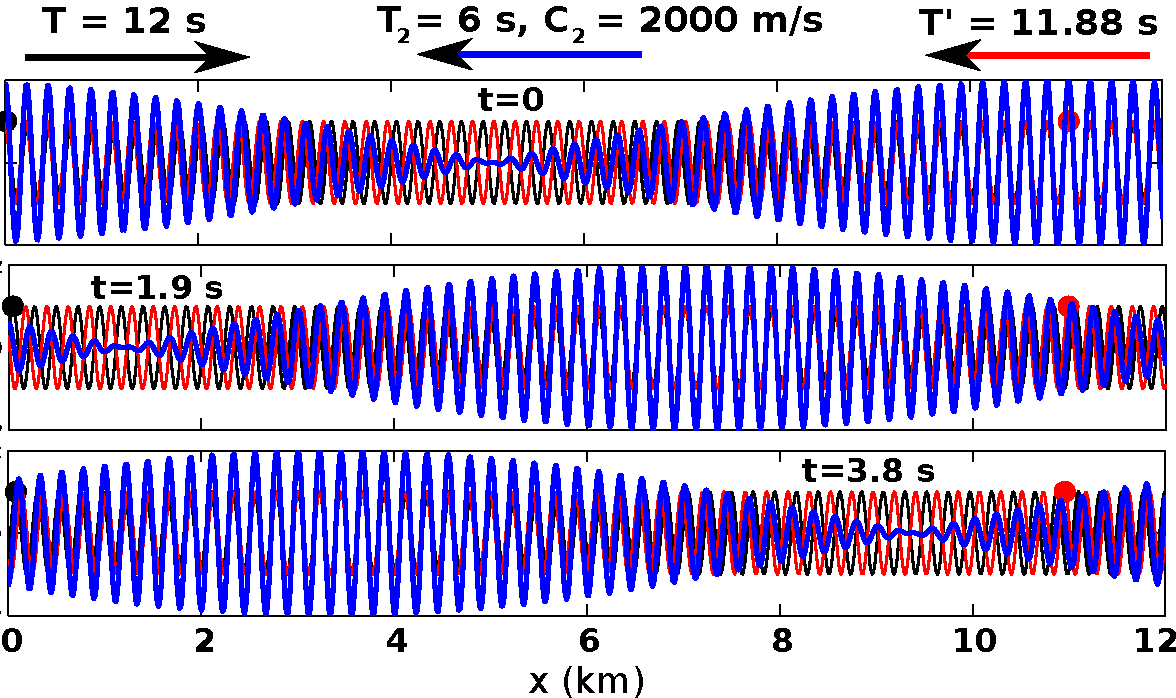
\includegraphics[width=0.9\textwidth]{FIGS_CH_SISMO/groupe_negatif.pdf}}
%\vspace{3.64in}
  \caption{Two wave trains with slightly different periods and propagating in opposite directions in deep water interfere to 
  form wave groups. The groups propagate in the same direction as the wave train which has the shorter wave  periods. 
  The red and black dots are attached to a crest of their monochromatic component, and these crests travel 100 times slower than the group.}
\label{fig:group_negative}
\end{figure}
%%%%%%%%%%%%%%%%%%%%%%%%%%%%%%%%%%%%%%%%%%%%%%%%%%%%%%%%%%%%%%%%%%%%%%%%%%%%%

It is also interesting to consider the pressure at the bottom. Indeed, for finite values of $kD$ the orbital velocity at the bottom 
induces a pressure oscillation given by the usual Bernoulli term,  that is equal to $-(u^2+w^2)/2$, which is out of phase with the surface wave groups, whereas 
$\widehat{p}_{2}$ is in phase. As noted by \cite{Ardhuin&Herbers2013}, these two terms exactly cancel in the limit $kD \rightarrow 0$, which is clear 
from the incompressible solution for the bottom pressure given by \cite{Herbers&Guza1991}.

\subsection{Sum for a continuous spectrum}
In the limit of a continuous spectrum, $2 \left|Z_{1,\kb}^{+}\right|^2 \rightarrow E(k_x,k_y) \mathrm{d}k_x \mathrm{d}k_y$. The factor 2 is there 
because we use only positive frequencies (i.e. single-sided spectra), namely we gather the variance of the components with amplitudes $Z_{1,\kb}^{+}$ and $Z_{1,-\kb}^{-}$. 
Liekwise the spectrum of  $\widehat{p}_{2}$ is, 
\begin{equation}
F_{p2}(\Kb,f_s) = 2 \lim_{\left|d \Kb\right| \rightarrow 0, df_s \rightarrow 0} \frac{\left|\widehat{p}_{2}(\Kb,f_s) \right|^2}
{\mathrm{d}k_{2x} \mathrm{d}k_{2y} \mathrm{d} f_s}, 
\end{equation}
where $\widehat{p}_{2}(\Kb,f_s)$ is the Fourier amplitude of  $\widehat{p}_{2}$ with wavenumber vector  $\Kb$  and frequency  $f_s$. 
We now replace with eq. (\ref{p2_amplitude}), and transform the ocean wave spectral density  $E(k_x,k_y)={ C_g} E(f)/({2 \pi k})$. Now using  $f_s = 2 f$, we get 
$\mathrm{d}k_x \mathrm{d}k_y /\mathrm{d} f_2= {\pi k}/C_g \mathrm{d} \theta$ et il vient, 
\begin{eqnarray}
     F_{p2}(\Kb,f_s)  &\simeq & 2 \rho_w^2 \sigma^4 \left[\frac{1}{2} + \frac{3}{2\tanh^2 \left(k D \right)} \right]^2 
     \int_{k_x,k_y > 0} E(k_x,k_y) E(-k_x+k_{2x},-k_y+k_{2y}) \frac{\mathrm{d}k_x \mathrm{d}k_y }{\mathrm{d} f_s}  \\
  &\simeq & 2 \rho_w^2 g^2 k^2 \tanh^2(kh)  \left[\frac{1}{2} + \frac{3}{2\tanh^2 \left(k D \right)} \right]^2 
     \int_{k_x,k_y > 0} E(f,\theta) E(f,\theta+\pi) \frac{C_g^2 \mathrm{d}k_x \mathrm{d}k_y }{k^2 4 \pi^2 \mathrm{d} f_s}  \\
&\simeq & \rho_w^2 g^2 \tanh^2(kD) \frac{k C_g }{ 2 \pi}  \left[\frac{1}{2} + \frac{3}{2\tanh^2 \left(k D \right)} \right]^2 
     \int_{0}^{\pi}  E(f,\theta) E(f,\theta+\pi)  \mathrm{d} \theta  \\
&\simeq & \rho_w^2 g^2 \tanh^2(kD) f_s \left(\frac{1}{4}+\frac{kD}{2 \sinh(2kD)} \right) \left[\frac{1}{2} + \frac{3}{2\tanh^2 \left(k D \right)} \right]^2 
     \int_{0}^{\pi}  E(f,\theta) E(f,\theta+\pi)  \mathrm{d} \theta  \nonumber\\
\label{p2_spectrum}
\end{eqnarray}

In the limit of deep water ($kD \gg 1$), and writing the directional wave spectrum as $E(f,\theta)=E(f) M(f,\theta) $, this becomes
\begin{equation}
F_{p2}(\Kb \simeq 0,f_s)=\rho_w^2 g^2  f_s   E^2(f)I(f)/2,
\end{equation}
where the `overlap intergral' $I$ was defined by \cite{Farrell&Munk2008} as 
\begin{equation}
I(f)=\int_{0}^{2 \pi}M(f,\theta)M(f,\theta+\pi)\mathrm{d}\theta.\label{eq:I}
\end{equation}

As a result, there are seismic waves generated at all frequencies, provided that some energy 
travels in  opposite directions. This is also true for capillary waves, although in that case the dispersion relation and 
surface boundary conditions are different  \citep{Farrell&Munk2008}. 
From an ocean wave perspective,$K$ is so small compared to $k$ that we can use $K=0$. 
However, for the seismic waves, the magnitude and direction of $K$ will determine the type of seismic wave and its direction. 
Indeed, $K=0$ correspond to $P$-waves than travel along the vertical. Because the spectrum $F_{p2}$ is nearly constant for seismic wavenumbers, 
all the different waves are actually generated at the same time from the same pressure force.  In this sense, the wave-induced forcing is equivalent 
to an oscillating point force at the sea surface. 

\subsection{Free solutions: Rayleigh waves}
\subsubsection{Motion in the water layer}
%%%%%%%%%%%%%%%%%%%%%%%%%%%%%%%%%%%%%%%%%%%%%%%%%%%%%%%%%%%%%%%%%%%%%%%%%%%%%
\begin{figure}[ht]
\centerline{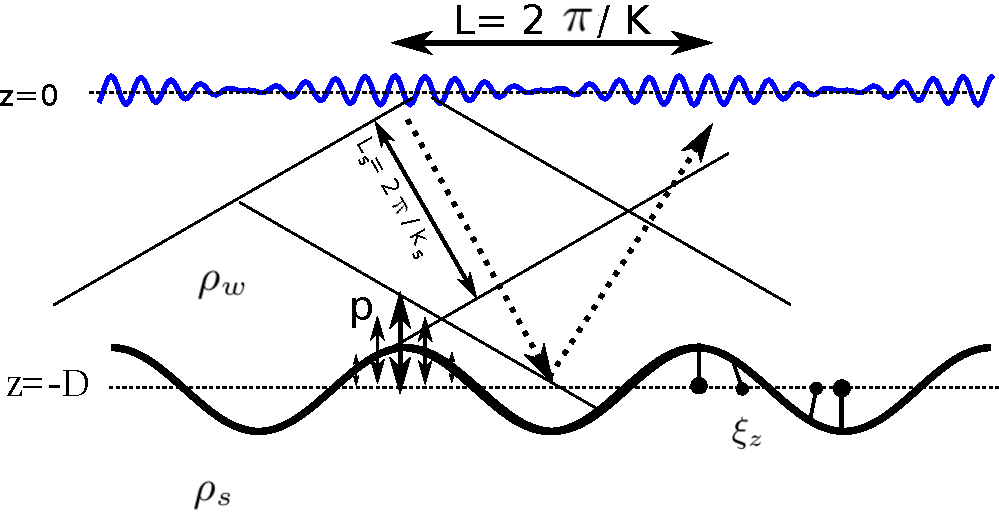
\includegraphics[width=0.7\textwidth]{FIGS_CH_SISMO/water_and_crust.pdf}}
%\vspace{3.64in}
  \caption{Schematic of wave group forcing acoustic waves in a water layer over a solid half-space. 
  The horizontal wavenumber $K$ is set by the forcing, whereas the true acoustic wavelength also involve the vertical 
  component $L_s=2\pi /k_s=2\pi /\sqrt{K^2+l_a^2}=\alpha_w/T$. The dashed arrows give the propagation direction of 
  acoustic waves in the water with the thin solid lines representing the surface of equal phase. 
  The superposition of up-going and down-going waves is a horizontally propagating mode. 
  In practice the angle of propagation of sound waves in Rayleigh modes is less than 65 degrees, as shown in figure \ref{fig:Rayleigh_dispersion}. }
\label{fig:water_and_crust}
\end{figure}
%%%%%%%%%%%%%%%%%%%%%%%%%%%%%%%%%%%%%%%%%%%%%%%%%%%%%%%%%%%%%%%%%%%%%%%%%%%%%

For a monochromatic wave of phase $\Theta = K x-\omega t$, the velocity potential is the real part of 
\begin{eqnarray}
 \phi = C \er^{l_a (z+h)} \er^{\ir \Theta}.
\end{eqnarray}
 with  $l_a$  a complex vertical wavenumber.  Replacing this solution in eq. (\ref{eq:acoustic_linear}) gives 
\begin{eqnarray}
 -\omega^2  + \alpha_w^2 \left( -K^2 +l_a^2 -  \frac{g}{\alpha_w^2} l_a\right)  & = & 0
\end{eqnarray}
with a solution
\begin{equation}
 l_a = \frac{  g}{2 \alpha_w^2} \pm l.
\end{equation}

The water motion is thus a superposition of two terms with the two possible signs, 
\begin{eqnarray}
 l= \sqrt{\frac{\omega^2}{\alpha_w^2} - K^2 + \frac{g^2}{4 \alpha_w^4}} \simeq \sqrt{\frac{\omega^2}{\alpha_w^2} - K^2}
\end{eqnarray}
giving
\begin{eqnarray}
 \phi = \er^{ g z/2\alpha_w^2 } \left ( C \er^{il(z+h)} + D \er^{-il(z+h)}\right) \er^{\ir \Theta} 
\end{eqnarray}
In the ocean  $\alpha_w \simeq 1500$~ m/s and $z > -11000$~m,  so that the term  ${ g z/2\alpha_w }$ 
varies between  0 et 0.02, and can be neglected for simplicity. 
For a supersonic forcing  ($\omega/K > \alpha_w$)  $l$ is real and we get acoustic waves, 
whereas a sub-sonic forcing ($\omega/K < \alpha_w$) gives evanescent waves, decreasing exponential from the sea surface. These are 
acoustic-gravity modes. 

\subsubsection{Motion in the solid Earth}
Treating the solid Earth as a homogenous medium with a compression velocity $\alpha_s$ and shear velocity $\beta$, given 
by the Lam{\'e} coefficients of the solid, 
\begin{eqnarray}
  \alpha_s^2& =&\frac{\lambda+2 \mu}{\rho_s}, \\
  \beta^2& =&\frac{\mu}{\rho_s}.
\end{eqnarray}
The elasticity equation gives Laplace's equation for the 
velocity potential  $\phi_s$ and the stream function  $\psi$. With the same phase as in the water, $\Theta = k x-\omega t$ 
a finite amplitude at $z \rightarrow - \infty$ gives solutions of the form 
\begin{eqnarray}
  \phi_s &=&  A \er^{m(z+h)}\er^{\ir \Theta}, \\
  \psi   &=& B  \er^{n(z+h)}\er^{\ir \Theta}. 
\end{eqnarray}

The vertical wavenumbers $m$ and $n$ are given by the generalized Bernoulli equation, 
\begin{equation}
%\delta_x = \frac{\alpha_s^2}{\omega^2}    \er^{\ir \Theta}
m = \frac{\ir g}{2 \alpha_s}+\sqrt{K^2 - \frac{\omega^2}{\alpha_s^2} - \frac{g^2}{4 \alpha_s^2}}
       \simeq \sqrt{K^2 - \frac{\omega^2}{\alpha_s^2}}  \quad {\mathrm{and}} \quad  
n \simeq \sqrt{K^2 - \frac{\omega^2}{\beta^2}},
\end{equation}
where $A$ and $B$ are the two constant amplitudes of the velocity potential and streamfuction, 
that have units of  m$^2$/s. These two unknowns 
are given by the boundary conditons. 

Hence, the horizontal and vertical displacements are given by the real parts of 
\begin{eqnarray}
%\delta_x = \frac{\alpha_s^2}{\omega^2}    \er^{\ir \Theta}
\xi_x &=&  \left(K A  \er^{m(z+h)}      + \ir n B  \er^{n(z+h)}\right)  \er^{\ir \Theta} \label{eq:sismo_xi_x}/\omega, \\
\xi_z &=&    \left(- \ir m A  \er^{m(z+h)} +  K B  \er^{n(z+h)} \right) \er^{\ir \Theta} /\omega \label{eq:sismo_xi_z}
\end{eqnarray}
The first term is a compression wave with a velocity field
$u_A =\partial \xi_x /\partial t = \partial \phi_s / \partial x$, 
avec $\phi_s =  A \er^{m(z+h)}\er^{\ir \Theta} $. 
The second term is a shear wave with a velocity field 
$u_B =\partial \xi_x /\partial t = -\partial \psi / \partial z$. 


Coupling at the water-solid interface requires to express the stresses in the solid using Hooke's law, which states that the 
stress is linearly related to the strain,
\begin{eqnarray}
\tau_{zz}   &=& \lambda \left(\frac{\partial \xi_x}{\partial x} + \frac{\partial \xi_z}{\partial z}\right) + 2 \mu \frac{\partial \xi_z}{\partial z}, \\
\tau_{xz}   &=& \mu  \left(\frac{\partial \xi_x}{\partial z} + \frac{\partial \xi_z}{\partial x}\right).
\end{eqnarray}
In our case we consider that the water freely slips over the solid, so that the shear stress 
at the bottom is  $\tau_{xz} = 0$ at $z=-h$. Using  (\ref{eq:sismo_xi_x})--(\ref{eq:sismo_xi_z}) we get, 
\begin{eqnarray}
 B= \frac{2 \ir K m}{n^2+K^2} A.
\end{eqnarray}
This relationship is characteristic of Rayleigh waves. 

\subsubsection{Coupling of water and solid Earth and pseudo-Rayleigh waves}
The boundary condtions $w_+=  w_-$ and $\tau_{zz} + p=0$ give the following relations that couple the amplitudes  
$A$, $C$ and $D$, 
\begin{eqnarray}
 A   (m - \frac{2 K^2 m}{n^2+K^2}) - \ir l E + \ir l F &= &0, \\
 A \frac{\ir}{\omega} \left[ - \rho_s  m^2 \alpha_s^2  
             + \lambda  K^2 + 4 \mu \frac{K^2 m n}{n^2+K^2} \right] - \ir \omega  {\rho_w} E - \ir \omega {\rho_w} F &=& 0.
\end{eqnarray}
Replacing $\lambda$ and $\mu$ by their expression in terms of  $\alpha_s$ and $\beta$, this gives
\begin{eqnarray}
 A   \frac{m \omega^2}{\omega^2-2K^2 \beta^2} - \ir l E + \ir l F &= &0, \\
  A \frac{\ir}{\omega \beta^2} \rho_s\left[- \frac{4 \beta^4 K^2 m n}{\omega^2- 2K^2 \beta^2} + \left(\omega^2- 2K^2 \beta^2 \right)\right]
 - \ir \omega  \rho_w E - \ir \omega \rho_w F &=& 0 
\end{eqnarray}

The last unknown, $\omega$ is now given by the sea surface boundary condition. Without forcing, this is 
$p(z=\zeta)=0 \simeq p(z=0)$, and it gives,  
\begin{eqnarray}
E =  B_2 \er^{-il h}, \\
F =  -B_2 \er^{il h},
\end{eqnarray}
and  
\begin{eqnarray}
   \frac{m \omega^2}{\omega^2-2K^2 \beta^2}   A - 2 \ir l  \cos(lh) B_2 &=& 0 \\
 \frac{\ir}{\omega \beta^2} \rho_s\left[- \frac{4 \beta^4 K^2 m n}{\omega^2- 2K^2 \beta^2} + \left(\omega^2- 2K^2 \beta^2 \right)\right]
 A - 2 \omega  {\rho_w} \sin(lh)_2 B  &=& 0.
\end{eqnarray}
The determinant of this linear system is thus zero, which gives 
the dispersion relation first given by \cite{Stoneley1926}, %dans le cas 
\begin{equation}
 \tan  \left(  l h \right)=    \frac{\rho_s}{\rho_w} 
\frac{l}{m} 
\times \frac{4 \beta^4 K^2 m n  - \left (\omega^2- 2  K^2 \beta^2 \right)^2   }{ \omega^4 }.\label{Rayleigh_dispersion}
\end{equation}
We also have
\begin{equation}
 B_2=m\frac{(n^2+K^2)-2K^2}{(n^2+K^2)\left(2 \ir l \cos(lh)\right)}A
=m \ir \frac{\omega^2}{(2 K^2 \beta^2 - \omega^2) 2  l \cos(lh)}A.
\end{equation}
The dispersion relation (\ref{Rayleigh_dispersion}) and motion are characteristic of Rayleigh waves, modified by a water layer. Because of this modification, these
are usually called pseudo-Rayleigh waves. 

The practical use of the dispersion relation is complicated by the presence of multiple solutions that are associated with different modes, 
%%%%%%%%%%%%%%%%%%%%%%%%%%%%%%%%%%%%%%%%%%%%%%%%%%%%%%%%%%%%%%%%%%%%%%%%%%%%%
\begin{figure}[ht]
\centerline{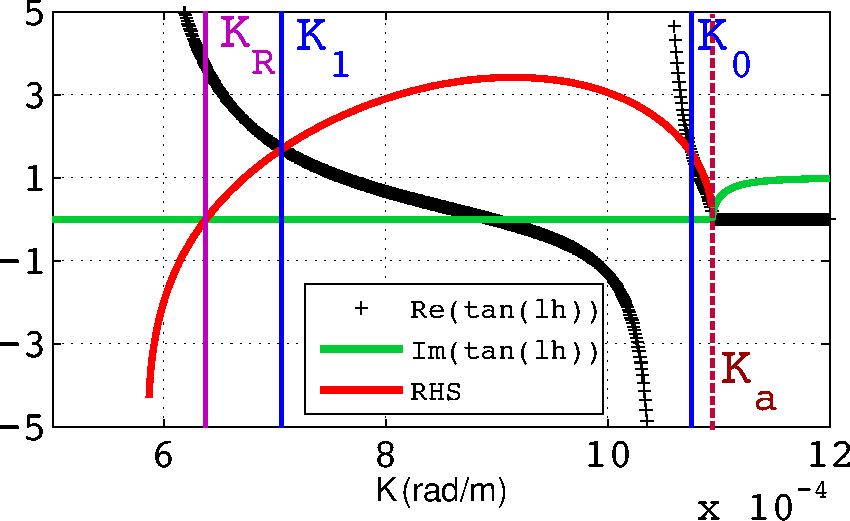
\includegraphics[width=0.7\textwidth]{FIGS_CH_SISMO/finding_roots_and_acoustic.pdf}}
%\vspace{3.64in}
  \caption{Real and imaginary parts of the left hand side 
  and real part of the right hand side of eq. \ref{Rayleigh_dispersion}. 
This calculation was performed for a water depth $D=5000$~m, with a sound speed in water of  $\alpha_w=1500$ m/s, a shear wave speed of  
$\beta=2800$m/s and water and crust densities of  1000 et 2500 kg/m$^3$. The chosen seismic frequency is $f_s=0.263$~Hz, 
corresponding to a non-dimensional depth $f_s h/\alpha_w=0.88$. 
The determinant of the system is zero for three values: one acoustic mode $K_a$ for which $l=0$ (horizontal propagation) and 
two seismic Rayleigh modes with wavenumbers $K_0$ and $K_1$. For non-dimensional frequencies below 0.34, only the 0 mode exists, 
and as the frequency increases, $K_0$ increases and new branches of  $\tan(lh)$ appear (in black) giving higher modes, that have a lower value 
of $K$. Besides, the zero of the right hand side (in red) gives the wavenumber of Rayleigh waves $K_R$ in the absence of a water layer.}
\label{fig:Rayleigh_roots}
\end{figure}
%%%%%%%%%%%%%%%%%%%%%%%%%%%%%%%%%%%%%%%%%%%%%%%%%%%%%%%%%%%%%%%%%%%%%%%%%%%%%

Figure \ref{fig:Rayleigh_roots} shows how different values of  $K$ are possible due to the multiple branches of the tangent function. 


The dispersion relation  \ref{Rayleigh_dispersion} is slightly different from that of Rayleigh waves without an ocean layer, 
which is 
\begin{equation}
\beta^4 K^2 m n  - \left (\omega^2- 2  K^2 \beta^2 \right)^2  =0.
\end{equation}
We also note that for large depths or short wavelengths  ($lh > 3 \pi / 2$) there are several solutions that 
correspond to different modes, each with a distinct motion pattern in the water column, while the pattern in the crust remains similar. 
Figure \ref{fig:Rayleigh_dispersion} shows the phase speed that are between the sound speed and the shear wave speed. 
For a given mode, the higher the frequency, the slower the horizontal propagation which tends to the sound speed. The acoustic part in the 
water thus propagate at shallower angles, becoming horizontal in the limit of high frequency. 

For high enough frequencies, the acoustic wavelength is much shorter than the water depth, and the variation 
in sound speed across the water layer can modify the propagation. In particular, nearly horizontal sound waves can 
be trapped in the SOFAR channel, and there can be a decoupling of the water layer and solid Earth. 
%%%%%%%%%%%%%%%%%%%%%%%%%%%%%%%%%%%%%%%%%%%%%%%%%%%%%%%%%%%%%%%%%%%%%%%%%%%%%
\begin{figure}[ht]
\centerline{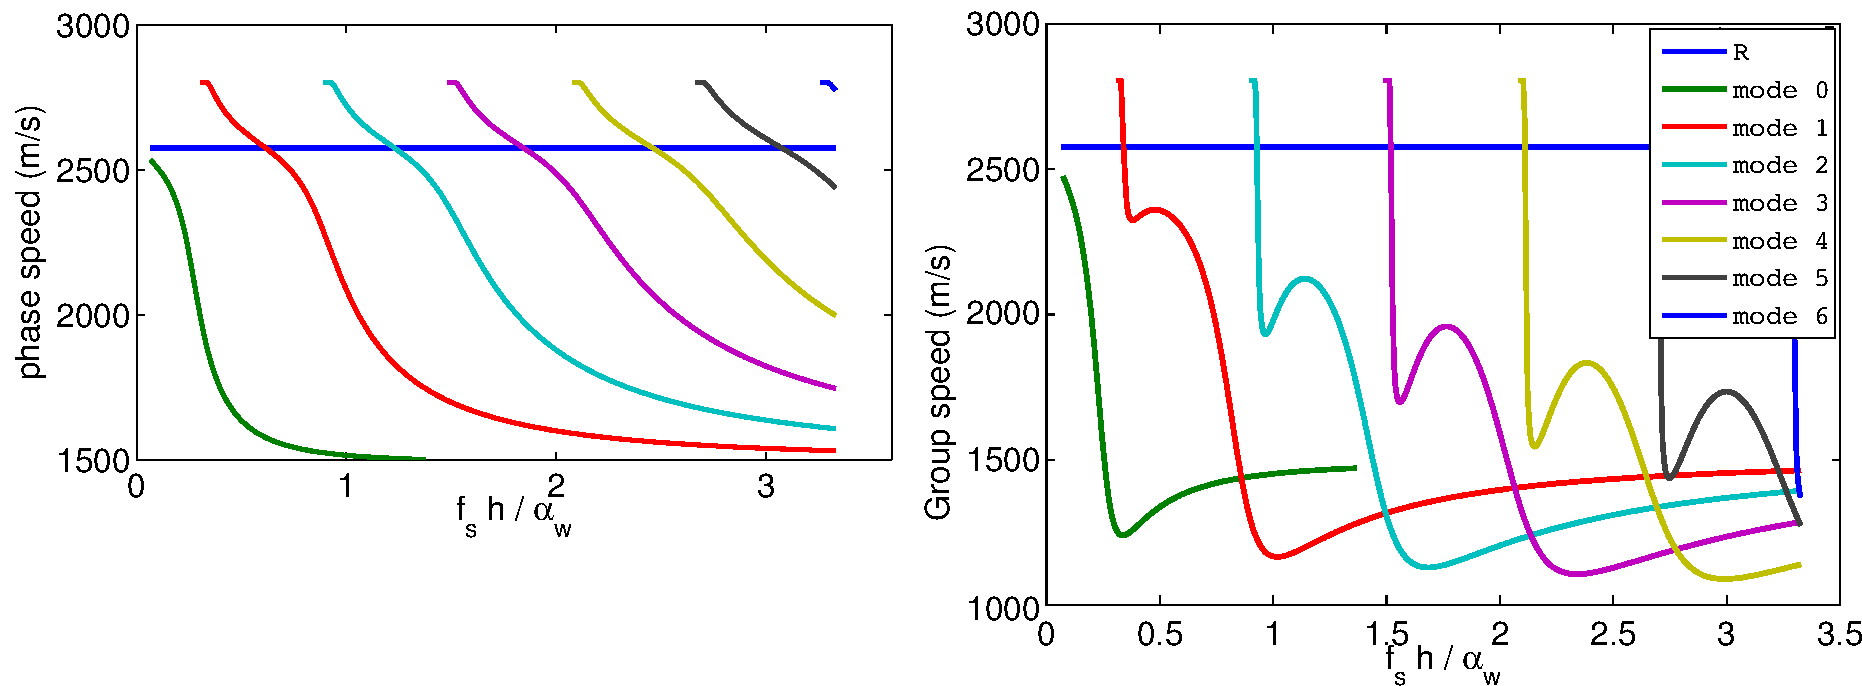
\includegraphics[width=\textwidth]{FIGS_CH_SISMO/Rayleigh_Cg_C.pdf}}
%\vspace{3.64in}
  \caption{Phase speeds and group speeds for Rayleigh waves in the presence 
  of a water layer. Calculations have been made with a water depth $D=5000$~m, a sound speed in the water $\alpha_w=1500$ m/s, a shear wave speed of  
$\beta=2800$m/s and water and crust densities of  1000 et 2500 kg/m$^3$.  Without the water layer the values are given by the blue line: 
in that case the Rayleigh waves are not dispersive. We have used seismic frequencies from 0 to 1~Hz, the latter value corresponding to $f_s h/\alpha_w=3.4$.  }
\label{fig:Rayleigh_dispersion}
\end{figure}
%%%%%%%%%%%%%%%%%%%%%%%%%%%%%%%%%%%%%%%%%%%%%%%%%%%%%%%%%%%%%%%%%%%%%%%%%%%%%

The angle of the acoustic propagation in the water are plotted for $D=5000$~m 
in  figure \ref{fig:Rayleigh_angle}, together with the vertical profiles of velocities in the water and crust. 
We note that the higher modes, with a lower $K$, penetrate deeper in the solid Earth. 
%%%%%%%%%%%%%%%%%%%%%%%%%%%%%%%%%%%%%%%%%%%%%%%%%%%%%%%%%%%%%%%%%%%%%%%%%%%%%
\begin{figure}[htb]
\centerline{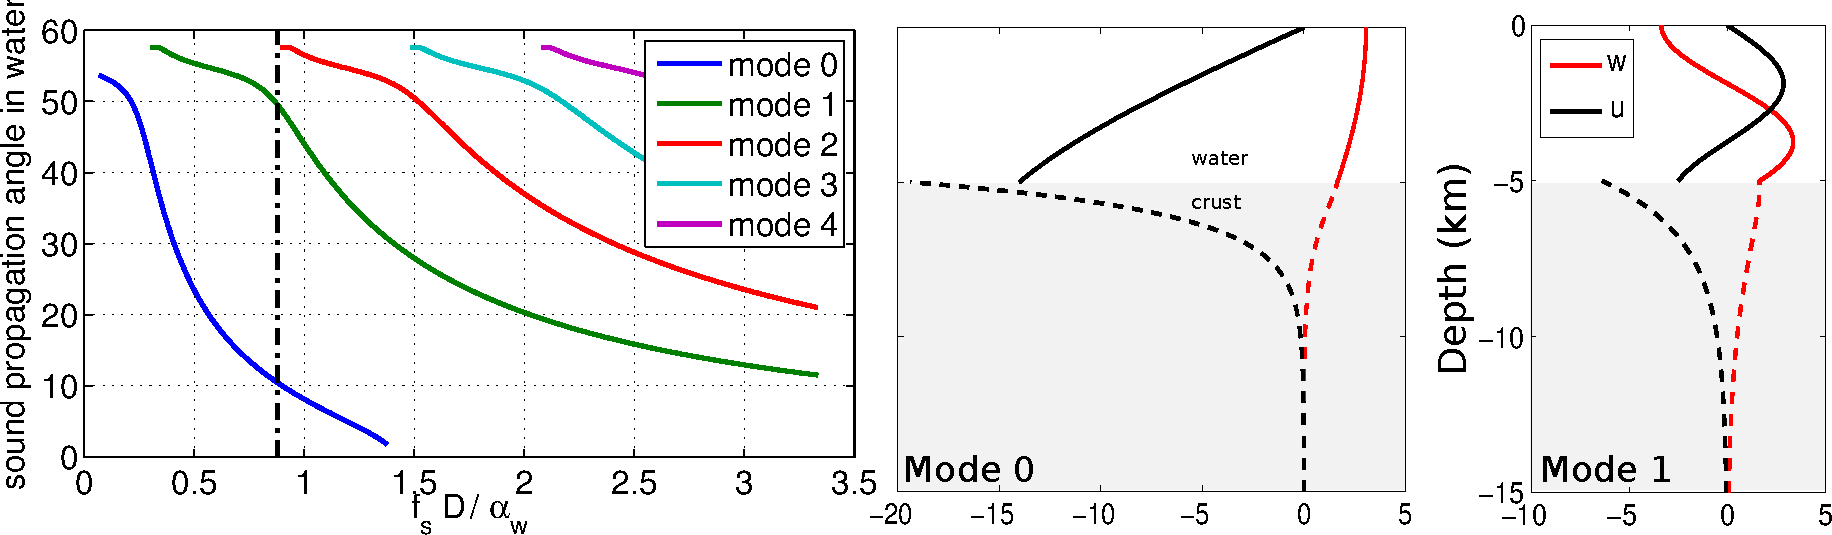
\includegraphics[width=\textwidth]{FIGS_CH_SISMO/Rayleigh_angle.pdf}}
%\vspace{3.64in}
  \caption{(a) Angle of propagation, relative to the hoizontal, of the two acoustic 
  waves that combine to make acoustic modes in the water. The vertical profile of the velocity amplitude for mode 0 and 1 and 
  $f_s D/\alpha_w=0.88$ are shown in the right panels. For modes 1 and higher, the vertical velocity is zero 
  at the nodes of the vertical standing acoustic wave. The zero-pressure level correspond to the zero-velocity levels,  
  in particular at the surface.}
\label{fig:Rayleigh_angle}
\end{figure}
%%%%%%%%%%%%%%%%%%%%%%%%%%%%%%%%%%%%%%%%%%%%%%%%%%%%%%%%%%%%%%%%%%%%%%%%%%%%%

\subsubsection{Displacements, pressure, velocity and energy in Rayleigh waves}
To finish with this description of Rayleigh waves, we can express 
all the wave-related quantities in terms of the ground displacement amplitude at the top of the crust  $\delta$,
\begin{eqnarray}
A &=& \frac{\omega^2-2k^2 \beta^2}{m \omega^2} \delta \\
 B&=& \frac{2 \ir k m}{n^2+K^2} A \\
B_2 &=& \frac{\ir \omega}{2 l \cos(lD)} \delta \\
\xi_z (z=-D) &=& \delta \cos \Theta \\
  \phi_s &=&  A \er^{m(z+D)}\er^{\ir \Theta} \\
  \psi   &=& B  \er^{n(z+D)}\er^{\ir \Theta} \\ 
\phi &=&  2 \ir l B_2 \sin(lz) \er^{\ir \Theta}  \\
p'(z)&=&  \Re\left[\ir \rho_w \omega \phi\right] =  - \delta \rho_w  \omega^2 \frac{\sin(lz)}{l\cos(lD)}  \cos \Theta.
\end{eqnarray}

From these we can evaluate the seismic wave energy per unit horizontal surface  $E_s$, taking twice the kinetic 
energy in both water and solid Earth, 
\begin{eqnarray}
E_s &=& \rho_w \int_{-D}^{0} \overline{\left(u^2+w^2\right)}  {\mathrm d}z + \rho_s \int_{-\infty}^{-D} \overline{\left(u^2+w^2\right)} {\mathrm d}z \\
 &=&  T_{E \delta}(D) \frac{\delta^2}{2} \quad \mathrm{with} \\
T_{E \delta}(D) &=& \rho_s \left[\frac{(K B/A +m)^2}{2 m} +\frac{(n B/A+K)^2}{2 n}\right]\left(\frac{A}{\delta}\right)^2 \nonumber \\
                & & + \rho_w   \left\{ l^2 \left[2D+sin(2 lD)/l\right] +  K^2 \left[2D-sin(2 l D)/l\right]\right\}\left(\frac{B_2}{\delta}\right)^2
\label{Kedelta}
 \end{eqnarray}

\section{Forced solutions:  Acoustic-Gravity, Rayleigh and body waves}
\subsection{Matrix inversion}
Let us now consider what happens with the ocean wave forcing. 
The surface boundary condition is now  $p'=P \er^{\ir(K x - \omega t)}$ at $z=0$, and $p'=-\rho_w \partial \phi_2/\partial t + P_b \er^{\ir(K x - \omega t)}$ at the bottom. This is now analog to the problem 
of wave generation by the wind, treated in chapter  \ref{ch_Satm}. 

Boundary conditions are now, for $kD \gg 1$, and neglect $P_b$, 
\begin{eqnarray}
  E \er^{ilh} + F \er^{-ilh} &= & \frac{\ir P}{\rho_w \omega} \\
\frac{m \omega^2}{\omega^2-2k^2 \beta^2}  A   - \ir l E + \ir l F &= &0 \\
 \frac{-\rho_s}{\omega^2 \rho_w} \left[- \frac{4 \beta^4 k^2 m n}{\omega^2- 2k^2 \beta^2}
 + \left(\omega^2- 2k^2 \beta^2 \right)\right] A + E + F &=& 0 
\end{eqnarray}
or, in matrix form, 
\begin{equation}
M \begin{pmatrix}
A\\
E\\
F\\
\end{pmatrix} =\frac{\ir}{\rho_w \omega} \begin{pmatrix}
P\\
0\\
0\\
\end{pmatrix} 
\end{equation}

The solution of this system of equation is the sum of a the solutions to the 'homogenous 
system' (without forcing) and one particular solution with the forcing. That solution can be written 
using the determinant and co-factors od the matrix \footnote{For a linear system of three equations 
\begin{equation}
\begin{pmatrix} a &b &c \\  
d &e & f \\
g &h & i \\
\end{pmatrix}\begin{pmatrix}
A\\
E\\
F\\
\end{pmatrix} =\begin{pmatrix}
1\\
0\\
0\\
\end{pmatrix}, 
\end{equation} 
the determinant is 
\begin{equation}\det M = aei + bfg + cdh - ceg -fha -ibd \end{equation}
 and the first co-factor is  $ei-fh$ 
so that  $A=(ei - fh)/\det M$, and likewise $E=(fg - di)/\det M$ and $F=(dh - eg)/\det M$. }
 $M$
giving  
\begin{equation}
A= -2 l \ir P / \det M
\end{equation}
with 
\begin{equation}
\det M = \frac{2}{ \omega\left (\omega^2- 2  K^2 \beta^2 \right)}\left\{ l \rho_s \cos(lD) \left[4 \beta^4 k^2 m n - 
            \left (\omega^2- 2  K^2 \beta^2 \right)^2  \right]
   - \rho_w m \sin(lD) \omega^4 \right\}.
\end{equation}

\subsection{Four different types of waves and equivalent point force}
The amplitude of the seismic displacement 
as a function of the sea surface pressure amplitude 
in the form of a gain factor  $\delta= G(\omega) P(\omega)$, with the gain
\begin{equation}
G = \frac{2 l  m  (K^2-n^2 )}{(n^2+K^2)\omega \det M}.
\end{equation}

Contrary to the case without forcing, we can now have waves at all wavenumbers and frequencies, but their amplitude $G P$ varies 
as shown in figure \ref{fig:k_f_plot}. 
%%%%%%%%%%%%%%%%%%%%%%%%%%%%%%%%%%%%%%%%%%%%%%%%%%%%%%%%%%%%%%%%%%%%%%%%%%%%%
\begin{figure}[htb]
\centerline{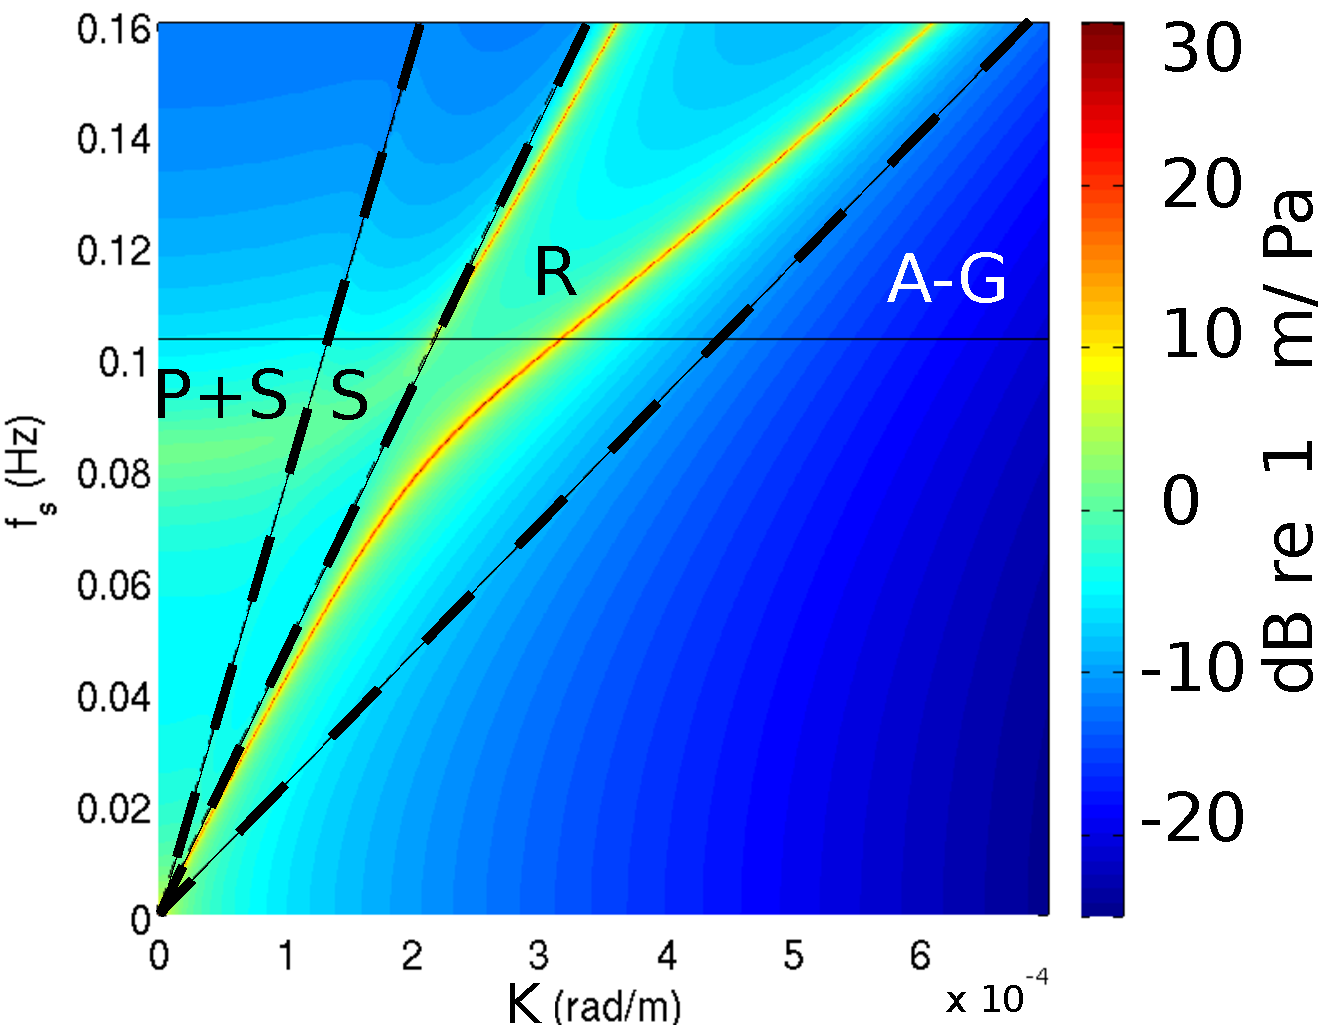
\includegraphics[width=0.7\columnwidth]{FIGS_CH_SISMO/k_f_plot.pdf}}
%\vspace{3.64in}
  \caption{Magnitude of the transfer function $G(K,f_s)$ illustrating the 
singularities along the dispersion relations of the free Rayleigh modes with wavenumbers $K=K_{n}(f_s)$, 
that correspond to $\det(M)=0$. The oblique 
dashed lines correspond to phase speeds equal to $\alpha_c$, $\beta$, and $\alpha_w$, and separate the four domains 
body waves (P+S), mixed body and evanescent waves (S), Rayleigh waves (R) and acoustic-gravity modes (A-G).
%The horizontal line separates 
}
\label{fig:k_f_plot}
\end{figure}
%%%%%%%%%%%%%%%%%%%%%%%%%%%%%%%%%%%%%%%%%%%%%%%%%%%%%%%%%%%%%%%%%%%%%%%%%%%%%
We can distinguish 4 different domains 
\begin{itemize}
  \item acoustic-gravity waves (AG) for $K/\omega < \alpha_w$: for a monochromatic forcing, these waves vanish exponentially with depth
  \item free and forced Rayleigh waves for  $\alpha_w < K/\omega < \beta$: the free waves are the ones with $\omega=\omega_r$
  \item evanescent $P$ waves and $SV$ body waves  for  $\alpha_s < K/\omega < \beta$: the $SV$ propagate down in the solid Earth 
  \item $P$ and $SV$ body waves for  $\alpha_s > K/\omega$: both $P$ and $SV$ propagate down in the solid Earth.
 \end{itemize}

Ocean waves are random and have a spectrum with a finite width which is typically much wider than the $K$'s of Rayleigh waves, so that waves at a given location excite, simultaneously, a broad range of wave numbers 
on the wavenumber plane, ans illustrated by figure \ref{fig:4domains}.
%%%%%%%%%%%%%%%%%%%%%%%%%%%%%%%%%%%%%%%%%%%%%%%%%%%%%%%%%%%%%%%%%%%%%%%%%%%%%
\begin{figure}[htb]
%\centerline{\includegraphics[width=\columnwidth]{schematic_fig1.eps}}
\centerline{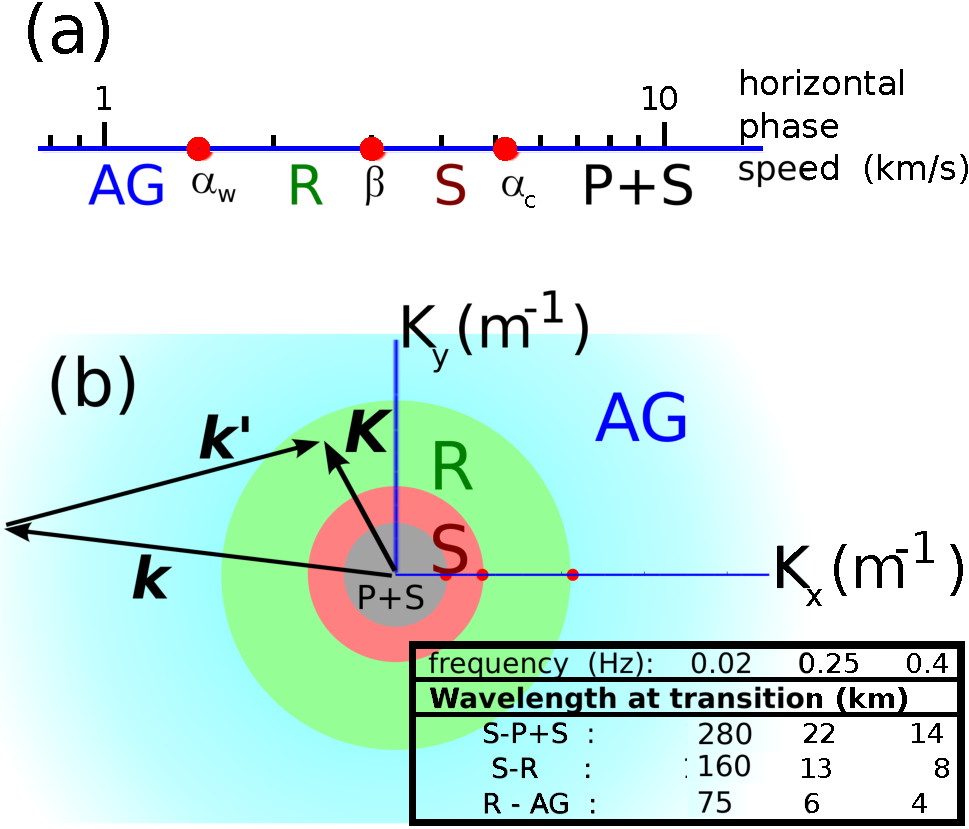
\includegraphics[width=0.55\columnwidth]{FIGS_CH_SISMO/schematic_fig1_v3.pdf}}
%\vspace{3.64in}
  \caption{(a) 
The vertical evanescent or propagating nature of the noise field in the solid and liquid layers is 
defined  by the horizontal phase speeds relative to the distinct values of the sound speed 
in the ocean ($\alpha_w$), and the shear ($\beta$) and compression ($\alpha_c$) speeds in the crust.
 From slow to fast, there are the acoustic-gravity (AG) domain, the Rayleigh (R) wave 
domain, and two body wave domains ($S$ only, and $P$ and $S$ together) 
(b)  For any fixed frequency, the four domains correspond to 4 concentric regions 
in the wavenumber plane. For three selected noise frequencies generated by  OSGW in the  infragravity, dominant and high frequency ranges of the forcing 
wave field, the limiting wavelengths between the four domains are indicated, using $\alpha_w=1.5$~km/s, $\beta=3.2$~km/s, 
$\alpha_c=5.54$~km/s. One example of interaction is shown with 
two gravity wave modes that interact to generate a Rayleigh wave  (black vectors, not to scale, $k$ and $k'$ should be much larger).}
\label{fig:4domains}
\end{figure}
%%%%%%%%%%%%%%%%%%%%%%%%%%%%%%%%%%%%%%%%%%%%%%%%%%%%%%%%%%%%%%%%%%%%%%%%%%%%%
The wave-induced pressure spectrum $F_p(K_x,K_y,f_s)$ waries smoothly around $K=0$ and is roughly constant for seismic wavenumbers. Thus, it is simimar to a white spectrum, corresponding 
to the spectrum of delta function in horizontal $(x,y)$ space. Hence, in terms of the power spectrum of the radiated waves, the ocean wavemotion is equivalent to a vertical oscillating force pushing on a single point of the sea surface with a root mean square value, 
\begin{equation}
F_{\mathrm{rms}} = 2 \pi \sqrt{F_{p}(K_x=0,K_y=0,f_s) dA d f_s},
\end{equation}
where $dA$ is the area over which the forcing is distributed and $d f_s$ is the frequency interval of interest. This 
equivalence is easy to show by computing the spectrum in $K_x,Ky$ of such a force, either directly as a delta function or as a pressure over a 
small square and taking the size of that square to zero. The spectrum of that force is equal to $F_{p}(K_x=0,K_y=0,f_s)$ for all values of $K_x$ and $K_y$, 
unlique the true effect of waves which becomes zero for large $K$. Also, compared to this point force, the phases of the different seismic modes are independant 
with real waves whereas they are identical with the point force. As a result, correlations of synthetic traces from a model forced 
by such point forces may be artificially high, where as power spectral densities should be alright. Such vertical forces were used by \cite{Gualtieri&al.2013} to 
model the seismic response, which contains all four types of waves, AG, R, P and S. We will now discuss these 4 types of waves. 

\subsection{Rayleigh waves}
For a given wavenumber $K$, there are one or several 
values of $\omega$ that gives a zero determinant, for which $G$ is infinite. Let us call $\omega_r$ one of these values, 
$\omega_r$ and $K$ are related by the Rayleigh wave dispersion relation 
(\ref{Rayleigh_dispersion}). 
In practice the wave forcing is continuous across frequencies and wavenumbers 
and characterized by a power spectral density $F_{p}(K_x,K_y,f)$, and in the case of the double-frequency source it is $F_{p2}(K_x,K_y,f)$ given by eq. (\ref{p2_spectrum}). It is thus possible 
to find the power spectrum of the ground displacement by integrating in frequency across these 
singularities, 
\begin{equation}
F_\delta(K_x,K_y) = \int_{0}^{\infty} \left|G\right|^2 F_{p3D}(K_x,K_y,\omega) {\mathrm d}{\omega}
\end{equation}
or in terms of seismic energy
\begin{equation}
F_E(K_x,K_y) = T_{E \delta}(D)  F_\delta (K_x,K_y) 
\end{equation}
with $ T_{E \delta}(D)$ given by (\ref{Kedelta}). 

Where the singularities in $G$ can be expanded at  $G=G'(\omega)/(\omega^2-\omega_r^2)$. 
Following Hasselmann (1962)%, see also chapter \ref{chwwscat})\nocite{Hasselmann1962},
 it is easy to prove that 
the response of a harmonic oscillator forced by  a continuous spectrum of density $F_p{K_x,K_y,\omega}$ with a singularity at $\omega = \omega_r$
integrates to a finite spectral density 
that grows linearly in time, giving a rate of change, 
\begin{equation}
\frac{\partial F_\delta(k_x,k_y)}{\partial t} =  S_{DF}(k_x,k_y)=\frac{\pi \left|G'\right|^2}{2 \omega_r^2}F_{p}(k_x,k_y,\omega_r).
\end{equation}

In practice we are often in a situation where the wave field changes slowly at the time scale of seismic propagation. 
In this quasi-stationary situation, assuming seismic energy conservation along rays, 
we have an energy balance similar to that of ocean waves, with conservation of the 
spectral densities in $K-$space, 
\begin{equation}
\mathbf{U} \bcdot \bnabla{F_{E}}(K_x,K_y) =  T_{E \delta}(h) S_{DF}(k_x,k_y),
\end{equation}
where $U$ is the group speed of seismic waves.
The seismic spectrum at point $s=0$ is given by the integral 
of sources along propagation rays with an along-ray distance $s$. 
Introducing the dissipation of seismic waves by anelastic processes, represented by a non-dimensional factor $Q$, we have
\begin{equation}
F_{\delta,0}(K_x,K_y)(K_{x}(0),K_{y}(0)) = \int_O^\infty \frac{T_{E \delta}(s)}{T_{E \delta}(0)} \frac{S_{DF}(K_{s}(s),K_{y}(s))}{U(s)}
 \exp\left[-\int_0^{s'} \frac{\omega}{U(s')Q(s')} {\mathrm d}s'\right] \mathrm{d} s
\end{equation}
%%%%%%%%%%%%%%%%%%%%%%%%%%%%%%%%%%%%%%%%%%%%%%%%%%%%%%%%%%%%%%%%%%%%%%%%%%%%%
\begin{figure}[htb]
\centerline{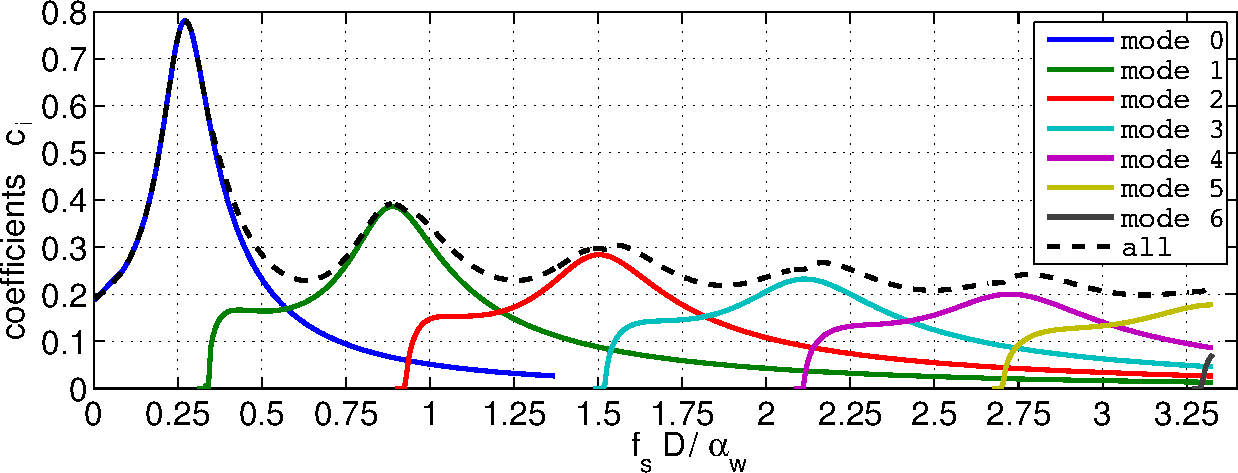
\includegraphics[width=\textwidth]{FIGS_CH_SISMO/Rayleigh_cn.pdf}}
%\vspace{3.64in}
  \caption{Non-dimensional coefficients $c_i$ and $\widetilde{C}$. 
  We note that the peaks of modes $i=0$ and $i=1$ occur for depths $D$ that are close to but slightly larger than   $D$ 
 $0.25+i/2$ the acoustic wavelength, just like the resonant modes of an oran pipe. In fact $c_i$ is maximum for a depth  that is 
 exactly $0.25+i/2$ the \emph{vertical} wavelength: because the propagation direction is oblique in the water, what is important for a maximum $c_i$ 
 is the constructive interference of these waves that reflect on the bottom and surface. This figure was drawn for  $\alpha_w=1500$~m~s$^{-1}$ 
 and $\beta=2800$~m~s$^{-1}$. 
The peak of $c_0$ is higher for larger values of  $\beta/\alpha_w$, which is similar to the impedance ratio of the bottom 
that defines the reflection of waves at the bottom. For example, changing $\beta$ to   $3200$~m~s$^{-1}$, the maximum value of $c_0$ is 1.03.}
\label{fig:sismo_coef}
\end{figure}
%%%%%%%%%%%%%%%%%%%%%%%%%%%%%%%%%%%%%%%%%%%%%%%%%%%%%%%%%%%%%%%%%%%%%%%%%%%%%

It is more convenient to work in azimuth and frequency 
because frequency is conserved during propagation.
For the Rayleigh mode number $i$ we have 
\begin{equation}
 F_{\delta,0}(\omega,\theta_s) =  \frac{K(0)}{U(0)} F_{\delta,0}(K_{x}(0),K_{y}(0)).
\end{equation}
To simplify our equations we will now assume that $Q$ is independent of the distance along the ray $s$, and we get 
\begin{equation}
 F_{\delta,0}(\omega,\theta_s) = \int_O^\infty \frac{S_{DF}(\omega)}{U(s)} \exp\left[-\frac{\omega}{Q} t(s)\right] \mathrm{d} s
\end{equation}
where $t(s)$ is the travel time (propagation time) and 
\begin{equation}
 S_{DF}(\omega)=\frac{k(0)}{U(0)} \frac{T_{E \delta}(s)}{T_{E \delta}(0)} \frac{S_{DF}(k_x,k_y)}{U(s)}.
\end{equation}
This source is a source of the power spectral density of the vertical 
elevation variance at point 0, per unit propagation length along a seismic ray. It thus has units of distance times time (m s). 

Equations are more simple when this source is written per unit propagation distance 
\begin{eqnarray}
 S_{DF}(\omega)&=&\frac{K(0) U(s)}{U(0) K(s)} \frac{T_{E \delta}(s)}{T_{E \delta}(0)} \frac{K(s) S_{DF}(K_x,K_y)}{U^2(s)}\\
               &=& \frac{K(0) U(s)}{U(0) K(s)} \frac{T_{E \delta}(s)}{T_{E \delta}(0)} 
               \frac{ 2 \pi \omega c^2_i}{\beta^5 \rho_s^2} F_{p3D}(K_x,K_y,\omega)
\end{eqnarray}
where $c_i$ is a non-dimensional coefficent that is a function of the non-dimensional depth $\omega D/\alpha_w$ and the seismic mode index $i$, 
\begin{equation}
c_i  =  \sqrt{\frac{\beta^5 \rho_s^2 k_i}{ U_i^2 2 \pi \omega } \frac{\pi \left|G_i'\right|^2}{2 \omega^2}}\label{eq:sismo_c_n}.
\end{equation}


Going to an extreme simplification, we will assume that  $U$ and $K$ are independant of  $i$ and $D$. 
The seismic source is thus of the order of 
\begin{equation}
S_{DF}(f_s) \simeq  \frac{2 \pi \omega  \widetilde{C}^2}{\beta^5 \rho_s^2} F_{p3D}(k_x,k_y,f_s).
\label{eq:sismo_SDF}
\end{equation}
where $\widetilde{C}$ combines all the $c_i$ values 
\begin{equation}
\widetilde{C}^2 =  \sum_{i=0}^{\infty} c_i^2.
\end{equation}
The values of  $c_i$ are obtained by finding the roots of the dispersion relation and using eq. (\ref{eq:sismo_c_n}). 
This gives values such as given in figure (\ref{fig:sismo_coef}).  When combining all modes the coefficient $\widetilde{C}$ varies with the 
ration of the vertical acoustic wavelength and the water depth $D$. 

\subsection{body waves}
A first theory  of body wave generation by ocean waves  was proposed by \cite{Vinnik1973}, who found that in some regions far from the ocean, the recorded microseism signals 
were dominated by body waves and not by surface Rayleigh waves. Since that time, many observations of body waves have been performed \citep[e.g.][]{Zhang&al.2010b,Obrebski&al.2013}. 
The theory of Vinnik did not include the important effect of the water layer. This was corrected by \cite{Ardhuin&Herbers2013} who simply applied the \cite{Hasselmann1963c} theory. 
This theory can explain both P and SV waves, but not the transversally polarized SH waves observed by \cite{Nishida&Takagi2016}, which probably require some bottom slopes or mode conversion. 
The following theoretical expression for the spectrum of $P$ waves was also derived by \cite{Gualtieri&al.2014}, and a first quantitative verification was performed by \cite{Farra&al.2016}. 


In the case of body waves, for $K/(2 \pi f_s) > \beta$, there are no singularities and thus the spectrum of the ground displacement is directly given by, 
\begin{equation}
F_{\delta,P}(f_s)= f_s   E^2(f)I(f)  \frac{\rho_w^2 g^2}{\rho_s^2 \beta_s^4 } c_P^2 
\label{eq:P_source}
\end{equation}
with a non-dimensional coefficient $c_{P}$,
\begin{equation}
 c_P^2=2 \pi \int_0^{\omega_s/\alpha_c} 
\frac{4 l^2 m^2 \rho_s^2 \beta_s^4}{\omega_s^2 \det^2 (M)} K {\mathrm d} K \label{c_P_def}.
\end{equation}


%%%%%%%%%%%%%%%%%%%%%%%%%%%%%%%%%%%%%%%%%%%%%%%%%%%%%%%%%%%%%%%%%%%%%%%%%%%%%
\begin{figure}[htb]
\centerline{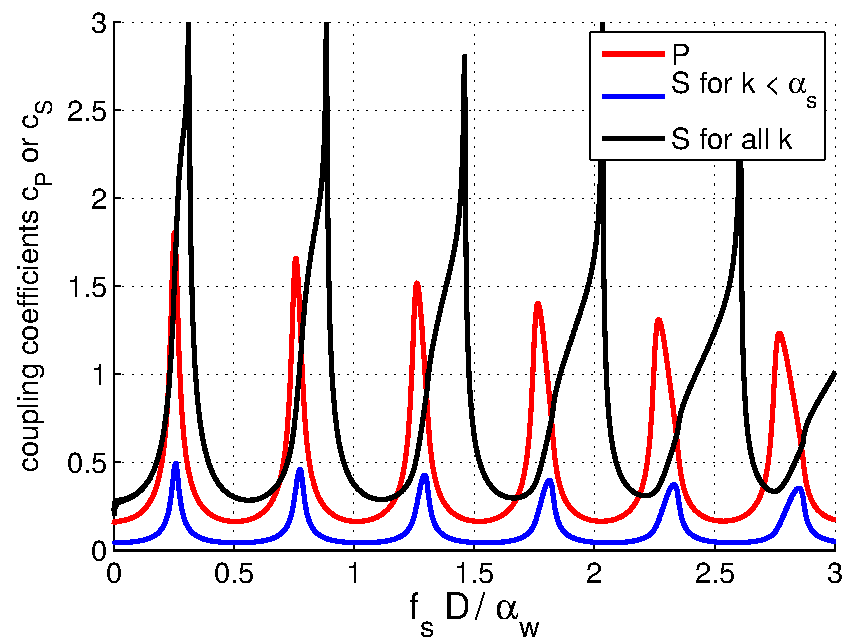
\includegraphics[width=0.7\linewidth]{FIGS_CH_SISMO/cp_cs.pdf}}
%\vspace{3.64in}
  \caption{Non-dimensionless coefficients  $c_P$ and $c_S$ that amplify the wave-induced pressure into ground displacement
associated with $P$ and $S$ waves.}
\label{fig:sismo_coefPS}
\end{figure}
%%%%%%%%%%%%%%%%%%%%%%%%%%%%%%%%%%%%%%%%%%%%%%%%%%%%%%%%%%%%%%%%%%%%%%%%%%%%%
A similar expression can be written for $S$ waves, and both are illustrated in 
figure  \ref{fig:sismo_coefPS}, 
\begin{equation}
F_{\delta,S}(f_s)= f_s   E^2(f)I(f)   \frac{\rho_w^2 g^2  }{\rho_s^2 \beta_s^4 } c_S^2.
\label{eq:S_source}
\end{equation}

 However, in the range of wavenumbers 
where $S$ waves exist, $k < \omega_s/\beta$, there can also be evanescent $P$ waves, and the system can approach the 
singularity for $\omega_s=\omega_{s,j}$ and $k=\omega_s/\beta$. We evaluated numerically the coefficient 
\begin{equation}
 c_S^2=2 \pi \int_0^{\omega_s/\beta} 
\frac{4 l^2 m^2 k^2 \rho_s^2 \beta_s^4}{\omega_s^2 (n^2+k^2)\det^2 (M)} K {\mathrm d} K.
\end{equation}

It is striking that the maxima of the coefficients $c_P$ and $c_S$ are much more pronounced that that of $c_i$ for Rayleigh waves,shown in figure \ref{fig:sismo_coef}. This is probably due 
the fact that, in  the case of $P$ and $S$ waves, the acoustic waves in the water are propagating closer to the vertical, with a narrow range of angles.  As a result, the spatial distribution 
of sources of body waves is much more constrained by the water depth, and should focus on smaller regions \citep{Obrebski&al.2013}. 
%%%%%%%%%%%%%%%%%%%%%%%%%%%%%%%%%%%%%%%%%%%%%%%%%%%%%%%%%%%%%%%%%%%%%%%%%%%%%
\begin{figure}
\centerline{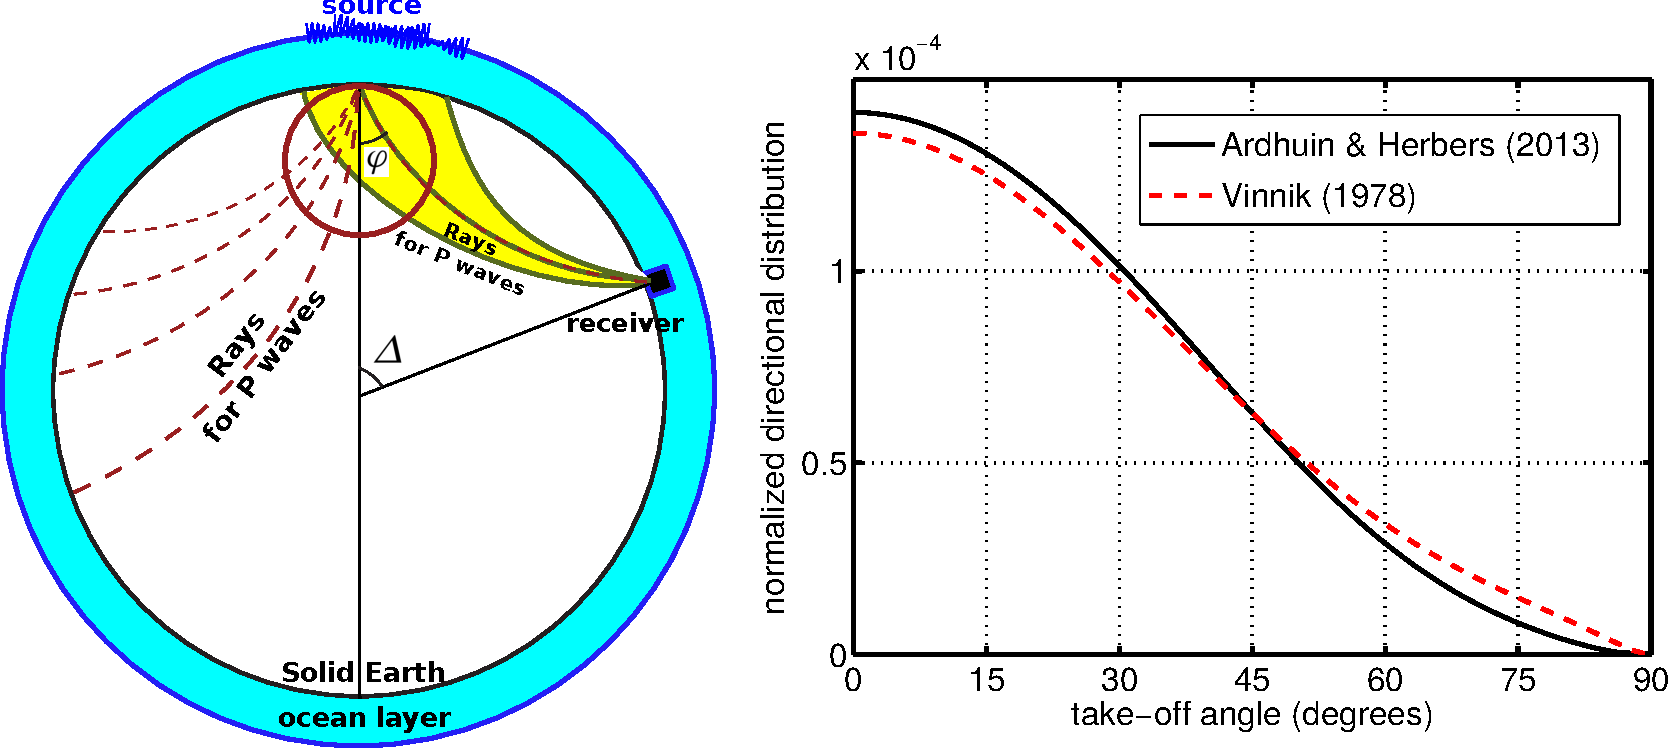
\includegraphics[width=\linewidth]{FIGS_CH_SISMO/C_P_phi.pdf}}
%\vspace{3.64in}
  \caption{Left: schematic of body wave propagation and definitions of take-off angle $\varphi$ and epicentric angle $\Delta$. Right: Dimensionless coefficients  $c_{P,\varphi}$ that amplify the wave-induced pressure into ground displacement. The 
maximum for a zero take-off angle corresponds to vertically propagating compression waves, and the compression waves that propagate 
along the crust have a vanishing amplitude.}
\label{fig:sismo_coef_CPphi}
\end{figure}
%%%%%%%%%%%%%%%%%%%%%%%%%%%%%%%%%%%%%%%%%%%%%%%%%%%%%%%%%%%%%%%%%%%%%%%%%%%%%

For the estimation of the spectrum recorded outside of a source area, it is more convenient to 
express the local seismic source as a function of the horizontal propagation angle $\theta$, and the vertical take-off angle 
$\varphi$. For $P$ waves, this gives, 
\begin{equation}
F_{\delta,P}(f_s,\theta,\varphi)= f_s   E^2(f)I(f)  \frac{1}{\rho_s^2 \beta_s^4 } c_{P,\varphi}^2 \sin \varphi
\label{eq:P_wave_at_source}
\end{equation}
with the non-dimensional coefficient $c_{P,\varphi}$ defined by 
\begin{equation}
c_{P,\varphi}^2=
\frac{4 l^2 m^2  \rho_s^2 \beta_s^4}{\omega_s \alpha_c  \det^2 (M)}\frac{\partial K}{\partial \varphi}, 
\end{equation}
which is the normalized source per unit solid angle $\Omega$, so that the average over the half space of downward directions 
${\Omega^-}$ is
\begin{equation}
c_P^2 = \int_0^{2 \pi} \int_0^{\pi/2} c_{P,\varphi}^2 \sin \varphi {\mathrm d} \varphi  {\mathrm d}\theta  =  \int_{\Omega^-} c_{P,\varphi}^2  {\mathrm d} \Omega
\end{equation}
as defined by eq. (\ref{c_P_def}). 

It is noteworthy that the distribution of the $P$-wave energy with the take-off angle is very  close to the 
one given by a small disk pushing at the top of a uniform half space, as given by \cite{Miller&Pursey1955} and used by 
\cite{Vinnik1973}, although it also varies with the non-dimensional water depth $f_s h/\alpha_w$. 
The only missing item in the work by \cite{Vinnik1973} is the very strong amplification of the motion 
for resonant frequencies associated with the water layer. Due to the large impedance contrast at the water-crust interface 
the relative amplification of $P$ waves is one order of magnitude stronger 
than for Rayleigh waves. We thus expect a much tighter correspondence of the strong seismic noise sources with 
the water depths that correspond to a maximum amplification. 


%%%%%%%%%%%%%%%%%%%%%%%%%%%%%%%%%%%%%%%%%%%%%%%%%%%%%%%%%%%%%%%%%%%%%%%%%%%%%
\begin{figure}
\centerline{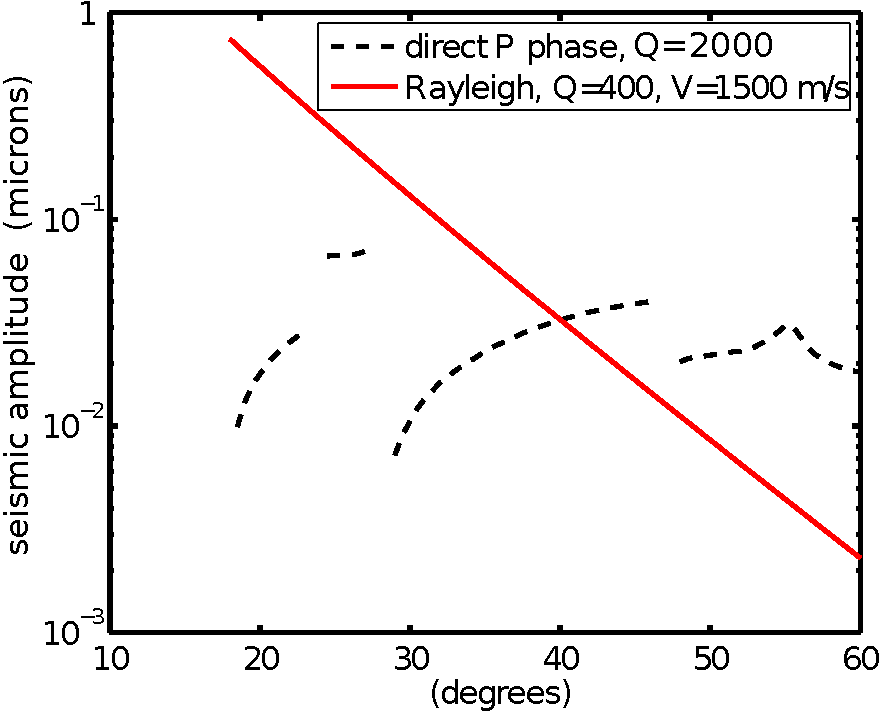
\includegraphics[width=0.7\linewidth]{FIGS_CH_SISMO/P_waves_vs_Rayleigh.pdf}}
%\vspace{3.64in}
  \caption{Estimates of the rms vertical ground displacement associated with Rayleigh or $P$ waves, 
as a function of the epicentric angle $\Delta$, for a source of intensity 
$\int F_{p2,\mathrm{surf}}(\Kb = 0,f) \mathrm{d}f = 4.2\times 10^4$ 
hPa$^2$~m$^2$ over a 330 by 330 km square, 
assuming an attenuation factor $Q=2000$ for the $P$ waves \citep{Pasyanos&al.2009}, with travel times 
given by the ak135 reference Earth model \citep{Snoke2009}. }
\label{fig:P_vs_Rayleigh}
\end{figure}
%%%%%%%%%%%%%%%%%%%%%%%%%%%%%%%%%%%%%%%%%%%%%%%%%%%%%%%%%%%%%%%%%%%%%%%%%%%%%
\cite{Ardhuin&Herbers2013} estimated that $P$ waves will dominate the signal at large distances from the source. 
The exact location where $P$-wave levels overtakes Rayleigh-wave levels depends 
on the relative attenuation of the two types of waves. With a realistic $Q=2000$ for the $P$ waves, and 
$Q=400$ for the Rayleigh waves, figure \ref{fig:P_vs_Rayleigh} shows that it occurs at an epicentric angle of $\Delta \simeq 40^{\circ}$, which is a distance of 4400 km, 
consistent with the observations reported by \cite{Vinnik1973} using Kazakhstan array data.  

\subsection{acoustic-gravity waves}
At the other end of the scale of forcing speeds, for $K/(2\pi f_s)< \alpha_w$, the response in the acoustic-gravity regime is also given by the local forcing. 

In order to illustrate the different types of solutions, it is interesting to evaluate the solution for an 
unbounded ocean, 
in which sound waves are radiated from the surface only. 
The velocity field and associated pressure fluctuations are 
\begin{eqnarray}
\phi_{2}&=& \frac{1}{\rho_w} \int  \frac{ \ir \omega_s \widehat{p}_{2}(\Kb,f_s) }{- \omega_s^2 +  \ir  g  l} \mathrm{e}^{\mathrm{i}\left[-lz +
    \Theta(\kb,\kpb,s,s')\right]}  {\mathrm d}\Kb   {\mathrm d}f_s 
 \\
p_{2}&=&\int   \frac{\widehat{p}_{2}(\Kb,f_s) }{1 - \ir g  l/\omega_s^2}  \mathrm{e}^{\mathrm{i}\left[-lz +
    \Theta(\kb,\kpb,s,s')\right]} {\mathrm d}\Kb   {\mathrm d}f_s  \label{eq:p2p}
\end{eqnarray}
where $p_{2}$ has been obtained using the linearized version of eq. (\ref{Bernoulli2}). The 
measured pressure signal is the sum of the linear pressure $p_1$, the second-order wave pressure $p_{2}$ given by eq. (\ref{eq:p2p}), and the 
Bernoulli correction $p_{2,B}$ given by
\begin{equation}
 p_{2,B}(z)= \rho_w \sum_{\kb,s,\kpb,s'}  D_{pb} \left(\kb,s,\kpb,s',z\right) Z_{1,\kb}^{s} Z_{1,\kpb}^{s'} 
 \mathrm{e}^{\mathrm{i}
     \Theta(\kb,\kpb,s,s')}\label{P2B}.
\end{equation}
We note that  $p_{2,\mathrm{bot}}$ defined in eq. (\ref{P2bot}) is equal to $p_{2,B}(z=-h)$. 

 
We shall neglect $  g |l|/\omega_s^2$, which is bounded by the ratio between the deep water gravity and sound speeds, which is less than 0.1 
for wave periods less than 180~s. We express
the velocity potential as a sum of propagating (acoustic, $l$ real) and evanescent (acoustic-gravity, $l$ imaginary) modes, 
\begin{equation}
   \phi_2 = \phi_{2,p} + \phi_{2,e}.
 \end{equation}

We get the frequency spectrum of the propagating modes by integrating over 
the inner regions of the wavenumber space (labelled P+S, S and R in figure \ref{fig:4domains}), 
\begin{eqnarray}
F_{p2,p}(f_s)=\int_{K < \omega_s/\alpha_w}  F_{p2,\mathrm{surf}}(\Kb ,f_s) {\mathrm d}\Kb   \label{Fp1Da}.
\end{eqnarray}
For this range of wavenumbers $|k-k'|< K <  \omega_s/\alpha_w$, and using the relations 
 $\omega_s \simeq 4 \pi f$ and, (for small $|f-f'|$), $|k-k'| \simeq 2 \pi |f-f'|/C_g \simeq 8 \pi^2 f |f-f'|$, 
we obtain an upper bound for the frequency difference $ |f-f'| <  g /(2 \pi \alpha_w)$ which is close to= 0.001~Hz. 
Typical ocean wave spectra have a relative frequency half-width $\sigma_f/f$ that is between 0.03 for swells and and 0.07 
for wind-seas \citep{JONSWAP}, 
so that $ E(f) \simeq E(f')$ 
is a good approximation for the interactions that drive long wavelength pressure fluctuations.


%In contrast, this approximation should lead to small overestimation of the noise level in the atmosphere, possibly 
%up to 1\%, as $\alpha_w$ is replaced by $\alpha_a$ giving a possible frequency mismatch 
%$\left|f-f'\right|$ as large as 0.005~Hz. Indeed, near the peak of the spectrum we generally have 
% $E^2((f+f')/2) > E(f) E(f')$. 


The wave spectrum is
thus broad enough for us to evaluate $ F_{p2,\mathrm{surf}}$ at $K=0$ using eq. (\ref{p2_spectrum}), 
and take it out of the integral in eq. (\ref{Fp1Da}). The acoustic spectrum simplifies to
\begin{equation}
F_{p2,p}(f_s)=\frac{\pi \omega_s^2}{\alpha_w^2} \rho_w^2 g^2  f_s   E^2(f)I(f)   \label{eq:noise_Lloyd}.
\end{equation}
This is identical to the expression given by \cite{Lloyd1981}. 


\subsubsection{Gravity noise in an unbounded ocean}
The pressure associated with acoustic-gravity modes is the other part of the integral in  (\ref{Fp1Da}), 
for $K > \omega_s/\alpha_w$.  The imaginary wave number $l$ gives a   
vertical attenuation of the power spectrum by a factor $ \er^{-2|l|z}$. 
With that attenuation we may, for large enough depths, 
  assume that only modes with $K \ll k$ contribute to the result,  so that we may take 
$F_{p2,\mathrm{surf}}(\Kb,f_s) \simeq F_{p2,\mathrm{surf}}(\Kb=0,f_s)$,  and take it out of the integrand. 
This approximation is valid only up to a maximum wave number $K_{\max}$ that is 
a small fraction of $k$, $K_{\max}=\epsilon k$. For numerical applications we used $\epsilon=0.2$. 

With this approximation we have, 
\begin{eqnarray}
F_{p2,e}(f_s,z)  &= & F_{p2,\mathrm{surf}}(\Kb=0,f_s) 2 \pi \int_{\omega_s/\alpha_w}^{K_{\max}}  K \er^{2|l|z} {\mathrm d} K   \nonumber \\
                 &  = &F_{p2,\mathrm{surf}}(\Kb=0,f_s) 2 \pi \int_{0}^{K_{\max}}  |l| \er^{2|l|z} {\mathrm d} |l|   \nonumber \\
                 &  = &\frac{\pi}{2 z^2}  \rho_w^2 g^2  f_s \left[1-\er^{2 z K_{\max}}\right]  E^2(f)I(f)    \label{Fp1Dag} 
\end{eqnarray}
A previous investigation by \cite{Cox&Jacobs1989} included an extra factor $(1 + z K_{\max})$ in front 
of the exponential term $\er^{2 z K_{\max}}$, because they neglected compressibility effects. 
That term , however, is negligible in the upper part of the water column, and their observations collected within 100 to 
290~m of the surface in 4000~m depth, are thus not affected by this small 
compressibility correction. 

%%%%%%%%%%%%%%%%%%%%%%%%%%%%%%%%%%%%%%%%%%%%%%%%%%%%%%%%%%%%%%%%%%%%%%%%%%%%%
\begin{figure}[htb]
\centerline{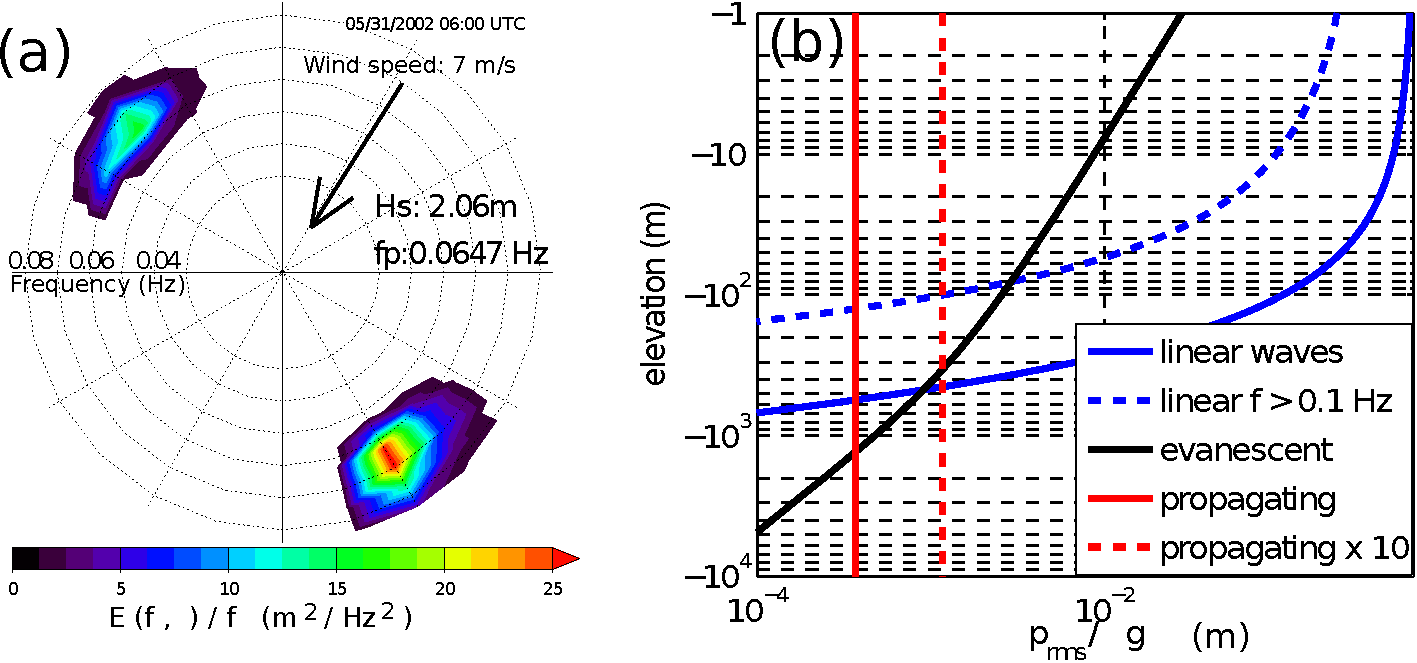
\includegraphics[width=\columnwidth]{FIGS_CH_SISMO/P_profiles_and_spec_v2.pdf}}
%\vspace{3.64in}
  \caption{Example of (a) directional wave spectrum and (b) 
resulting profiles of the different contributions to the pressure fluctuations in the ocean, 
assuming infinite water depth. 
The ratio of double frequency 
to linear wave contributions depends on the amplitude of the waves and on the directional spectral shape, 
because all double 
frequency contributions are proportional to $E^2(f)I(f)$. This directional spectrum was estimated with a numerical wave model, 
and corresponds to the loudest noise 
event recorded at the ocean bottom seismometer H2O, on 31 May  2002 at 25 N, 136 W. This unusual spectrum 
 has large wave energies in opposite directions, radiated from 
a North Pacific storm and Hurricane Alma \citep[This event is analyzed in detail by][]{Obrebski&al.2012}.}
\label{fig:P_profiles}
\end{figure}
%%%%%%%%%%%%%%%%%%%%%%%%%%%%%%%%%%%%%%%%%%%%%%%%%%%%%%%%%%%%%%%%%%%%%%%%%%%%%

As shown in figure \ref{fig:P_profiles}, the oceanic pressure signals can be dominated by linear gravity waves down to 
depths of a few hundred
meters. When looking at the double frequency band, linear waves may only dominate in the top 100~m. 
At these frequencies, the acoustic-gravity modes have the 
most important contribution between about 100 to 500~m, provided that $E^2(f) I(f)$ is large enough. Propagating modes 
should dominate only beyond about 1000 m in the case of an unbounded ocean, or only 300~m, when 
accounting for the reverberation in a finite depth ocean, assuming a typical tenfold amplification for a sea floor with realistic elastic 
properties\footnote{This amplification depends not only on the impedance ratio of the water and crust, which defines 
the amplification coefficients $c_j$ derived below, but also on the seismic attenuation coefficient $Q$, which is discussed in section 4. Realistic calculations following \cite{Ardhuin&al.2011} typically give a
factor 10 to 20 amplification of the sound in the water column due to the bottom elasticity.}. These depths will be reduced in the case 
of surface gravity waves with periods  shorter than the 15~s swells example shown in figure  \ref{fig:P_profiles}.

\subsubsection{Noise in a finite depth ocean}
For large depths compared to the OSGW wavelength, $kh \gg 1$, the finite depth 
has little effect on the evanescent modes except
for a doubling of the motion amplitude near the bottom, as the vertical profiles of the form 
$\exp(K z)$ are replaced by $\cosh(K z+K h)/\cosh(K h)$. This is similar to the finite depth effect 
on  linear wave motions. 
However, the propagating modes  radiated by the surface will now undergo multiple reflections at the bottom and sea surface, 
as shown in figure \ref{fig:water_and_crust}. The oceanic acoustic field is tightly coupled 
to elastic waves in the crust through these reflections.

One of the greatest complications induced by the presence of a bottom is the heterogeneity of  
the sediment and rock layers below the water column. 
The natural layering of the crust has a strong influence on the sound reflection and 
the nature of the seismic modes \citep[e.g.][]{Latham&Sutton1966,Abramovici1968}. 






\section{Modeling of seismic spectra using a numerical wave model}
While \cite{Hasselmann1963c} and \cite{Szelwis1982} already made some order of magnitude estimates of the microseism generated by 
realistic wave spectra, the first attempt using a numerical wave model was performed by \cite{Kedar&al.2008}. 

For a seismic frequency  $f_s=0.15$~Hz, the maximum of $\widetilde{C}$ corresponds to a depth $D\simeq2300$~m. This explains 
why oceanic ridges are generally stronger sources of microseisms at that frequency (figure \ref{fig:sismo_source}).

%%%%%%%%%%%%%%%%%%%%%%%%%%%%%%%%%%%%%%%%%%%%%%%%%%%%%%%%%%%%%%%%%%%%%%%%%%%%%
\begin{figure}
\centerline{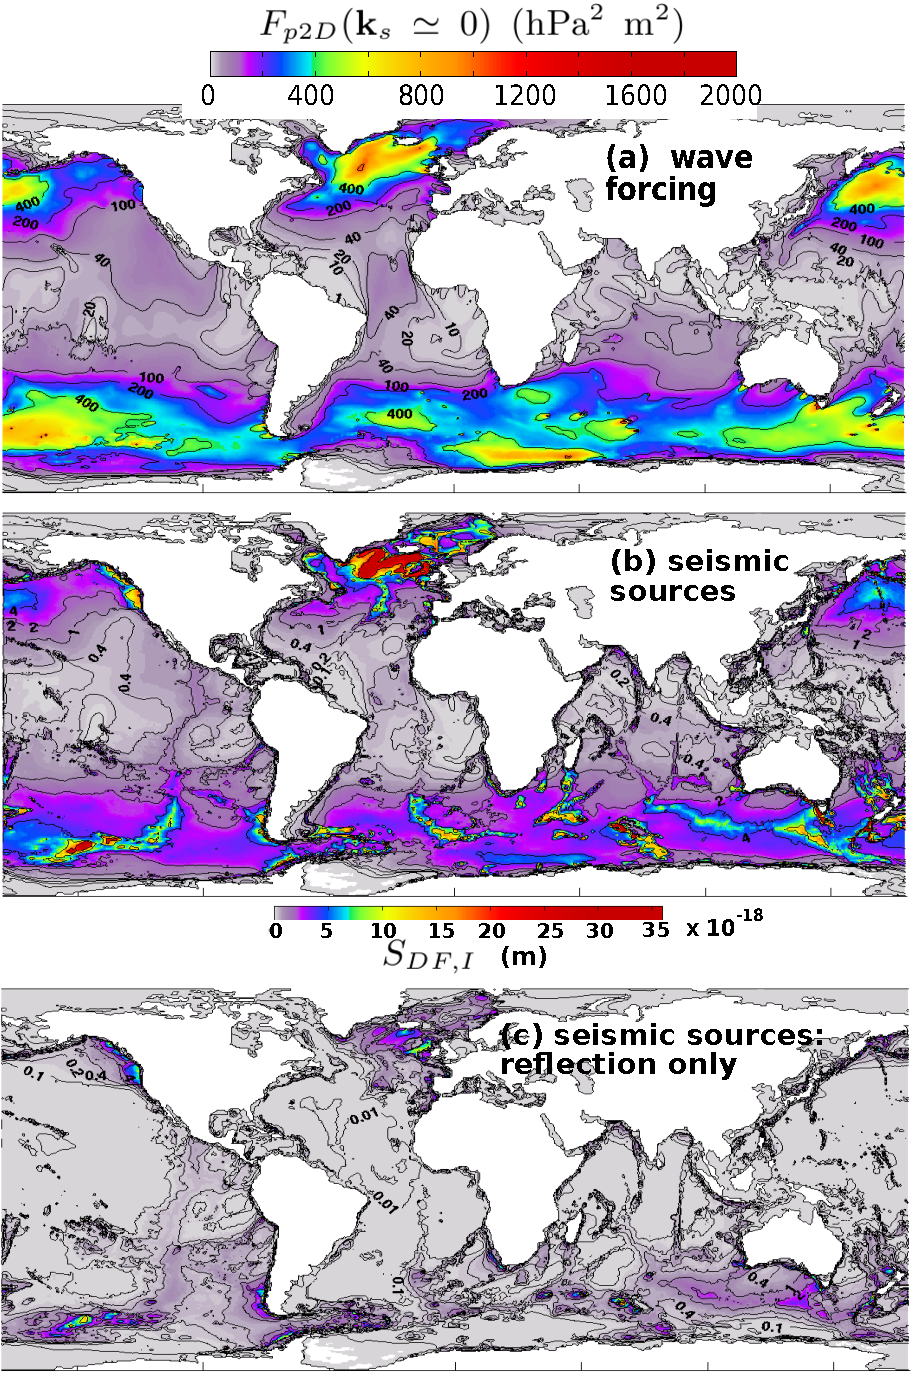
\includegraphics[width=0.8\textwidth]{FIGS_CH_SISMO/mean_sources_ref_noref_nobug.pdf}}
%\vspace{3.64in}
  \caption{Averaged microseism sources averaged over the year 2008 at global scales over the seismic frequency band 0--0.34~Hz, based on a numerical wave model 
\citep{Ardhuin&al.2011}. The top panel shows the average wave-induced pressure spectral density  
$F_{p2D}(k_x=0,k_y=0)=\int F_{p3D}(k_x=0,k_y=0,f_s) {\mathrm d}f_s$. The middle panel shows the seismic source, which combines the wave-induced pressure 
and the local amplification factor that varies with water depth
$S_{DF}(f_s)$. The bottom panel shows the contribution of coastal reflections only given as the difference of the model run with reflection and the model run without 
reflection. For reference, without scattering or dissipation a constant source of 10$\times 10^{-18}$ over a square with side length of 330~km gives 
an average amplitude $\delta_{\mathrm{rms}}^2=1\mu$m$^2$ at a distance of  1000~km.}
\label{fig:sismo_source}
\end{figure}
%%%%%%%%%%%%%%%%%%%%%%%%%%%%%%%%%%%%%%%%%%%%%%%%%%%%%%%%%%%%%%%%%%%%%%%%%%%%%

\subsection{Rayleigh wave propagation in a non-homogeneous medium}
Changes in water depth, as well as changes in sediment properties, have a large influence on the phase speeds and group speeds of seismic waves (figure \ref{fig:Rayleigh_dispersion}). We thus expect  that seismic waves are refracted and reflected. For $f_s=0.15$~Hz   Rayleigh waves typically speed up from phase speeds around $C_o=2000$~m/s with a water depth of 3000~m to  $C_c=2570$m/s. 

Besides, the amplitude of the vertical ground motion $\delta$ at the top 
of the crust is related to the energy flux. 
Without dissipation and neglecting reflections and lateral variations 
along   direction $y$, the evolution of $\delta$ along the $x$ direction 
between an ocean with a water depth $h$ and the continent is given by 
\begin{equation}
U(h_1) T_{E \delta}(h_1) \delta^2(h_1) = U(0) T_{E \delta}(0) \delta^2(0). 
\end{equation}
with $V(h_1)$ and $V(0)$ the group speeds over the ocean and over land, 
$T_{E \delta}(h_1)$ and $T_{E \delta}(0)$ being the transfer functions from the seismic energy to the vertical displacement at the top of the crust. 

Hence, just like waves propagating from deep 
to  shallow waters,
the variance of the displacement $\delta^2/2$ is amplified by a factor 
$U(h_1) T_{E \delta}(h_1) /(V(0) T_{E \delta}(0))$ that can be of the order of 
5 (figure \ref{fig:Rayleigh_shoaling}).
%%%%%%%%%%%%%%%%%%%%%%%%%%%%%%%%%%%%%%%%%%%%%%%%%%%%%%%%%%%%%%%%%%%%%%%%%%%%%
\begin{figure}
\centerline{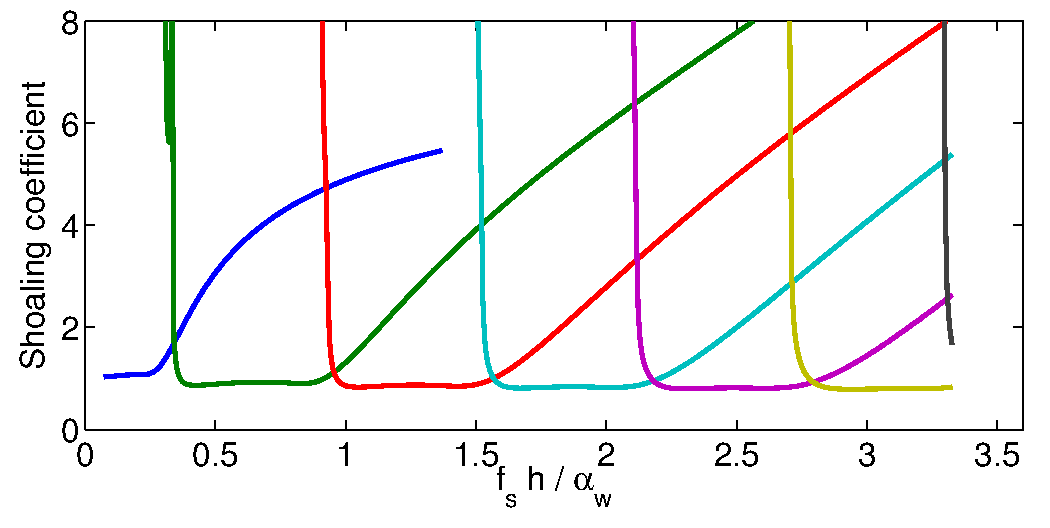
\includegraphics[width=0.7\textwidth]{FIGS_CH_SISMO/Rayleigh_shoaling.pdf}}
%\vspace{3.64in}
  \caption{Amplification coefficient for the vertical displacement variance at the top of the crust, when Rayleigh waves propagate perpendicular to shore from ocean to land, as a function of the ocean depth.}
\label{fig:Rayleigh_shoaling}
\end{figure}
%%%%%%%%%%%%%%%%%%%%%%%%%%%%%%%%%%%%%%%%%%%%%%%%%%%%%%%%%%%%%%%%%%%%%%%%%%%%%
As a result, the 0 mode progressively transforms into a continental Rayleigh wave. 

In the case of higher modes, they do not exist as such when the water depth goes below a critical value $h_c$. 
At these locations it is possible that they get transformed to mode 0.  
The real problem is made much more complex by the layering of sediments and rocks and their horizontal heterogeneity \citep{Gualtieri&al.2015}.

\subsection{Validation of modeled microseism}
The microseism sources add up along their propagation and their amplitude is modified by dissipation, scattering and refraction.  As a result, for a land-based station, nearby ocean sources have a stronger contributuon to the measured microseism than far away sources of equal power. Neglecting refraction effects, the only propagation effect taht we keep is the attenuation that we assume constant. 

This gives a power spectral density of the vertical ground motion for an observation longitude $\lambda$ and latitude $\phi$ that is the sum of sources over all oceans, 
\begin{equation}
F_\delta(\lambda,\phi,f_s)  =  \int_{- \pi/2}^{ \pi/2} \int_0^{2 \pi}\frac{S_{DF}(f_s)}{R_E \sin \alpha} ~ \mathrm{e}^{-2 \pi  f_s \alpha R_E / (V Q)}  (R_E^2 \sin \phi' {\mathrm d} \lambda' 
{\mathrm d} \phi')  \label{F_delta}\nonumber\\\end{equation}
where $V$ is the seismic group speed, and $Q$ is an attenuation factor. 
Taking  $V=1.8$~km~s$^{-1}$ and $Q=150$, the energy of seismic waves with frequency $f_s=0.15$~Hz is halved every 200 km. These two parameters are functions of the vertical structure and horizontal non-homogeneities of the Earth's crust. In particular $Q$ may have large variations from about 100 to 1000, primarily increasing with the age of the crust. 

For seismic stations located in  France  $Q \simeq 130$ gives a good agreement between model and observations for $f_s=0.14$~Hz 
(figure \ref{fig:sismo_mean_spec}.b), alors que pour certaines stations en Californie il faut reduire $Q$ to pres de 45 
(figure \ref{fig:sismo_mean_spec}.a). De faibles valeurs de $Q$ impliquent que l'essentiel du bruit sismique vient de regions tres proches 
de la station de mesure, les sources plus lointaines ayant ete fortement attenuees.
En Europe de l'ouest on estime que le bruit sismique est tout autant cause par les vagues qui passent sur la dorsale medio-Atlantique que par l'effet des 
reflections sur les coast Atlantiques. Les vagues en Mediterranee peuvent aussi be une source significative (figure \ref{fig:sismo_mean_spec}.c). 
%%%%%%%%%%%%%%%%%%%%%%%%%%%%%%%%%%%%%%%%%%%%%%%%%%%%%%%%%%%%%%%%%%%%%%%%%%%%%
\begin{figure}
\centerline{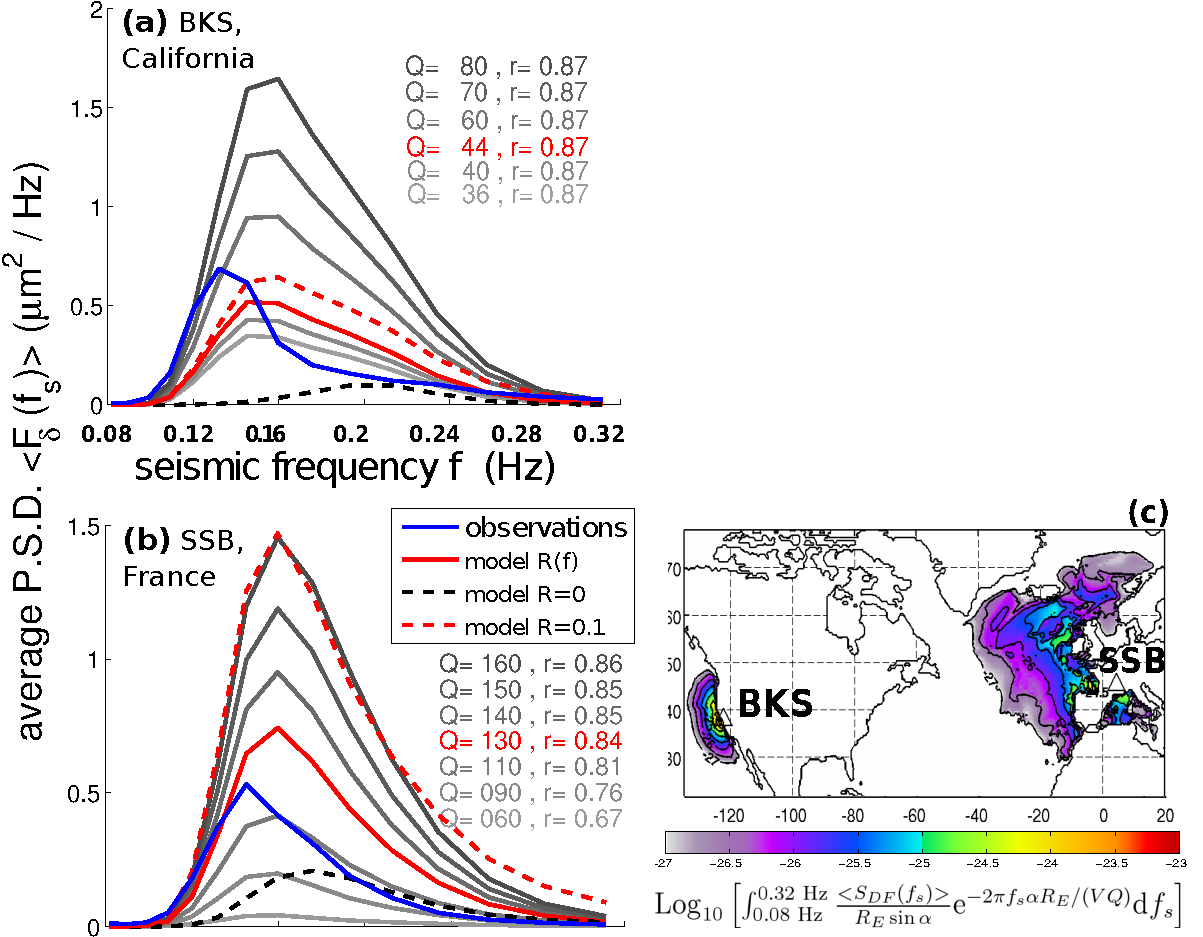
\includegraphics[width=\textwidth]{FIGS_CH_SISMO/mean_2008_sources_BKS_SSB_only.pdf}}
%\vspace{3.64in}
  \caption{(a et b) spectres moyens du deplacement sismique observe et modelise avec differentes valeurs du facteur de qualite $Q$. Pour la 
valeur optimale de $Q$ les resultat avec differentes modelisations de la reflection des vagues par la coast sont aussi montres: une 
reflexion constante de 10\%, pas de reflexion du tout ($R=0$) ou alors une reflection $R(f_s)$ variant lineairement avec la frequence. Dans le
cas de SSB cette variation est de $R=0.06$ pour $f_s=0.04$~Hz to $R=0.01$ at $f_s=0.15$~Hz et pour BKS cette reflexion est augmentee de 50\%. 
(c) Moyenne des contributions au bruit sismique pour l'annee 2008, pour les stations de Berkeley (BKS) et de Saint Sauveur en Rue (SSB), au sud 
de Saint-Etienne. 
}
\label{fig:sismo_mean_spec}
\end{figure}
%%%%%%%%%%%%%%%%%%%%%%%%%%%%%%%%%%%%%%%%%%%%%%%%%%%%%%%%%%%%%%%%%%%%%%%%%%%%%

Parce qu'il faut des vagues de same frequence mais de directions opposees pour generer du bruit sismique, les sources sont associees to des houles opposees 
la mer du vent, ou to la reflexion des vagues, to la coast ou par des icebergs. 
Avec un modele assez simple de la reflexion to la coast on peut simuler le bruit sismique de facon tres realiste. La principale inconnue etant 
l'attenuation des ondes sismiques lors de leur propagation. 

La figure \ref{fig:sismo_timeseries} montre la variation au cours de l'annee 2008 de l'amplitude du deplacement sismique vertical $\delta_{\mathrm{rms}}$
observe et modelise par l'equation (\ref{F_delta}) pour les stations SSB et BKS. 


%%%%%%%%%%%%%%%%%%%%%%%%%%%%%%%%%%%%%%%%%%%%%%%%%%%%%%%%%%%%%%%%%%%%%%%%%%%%%
\begin{figure}
\centerline{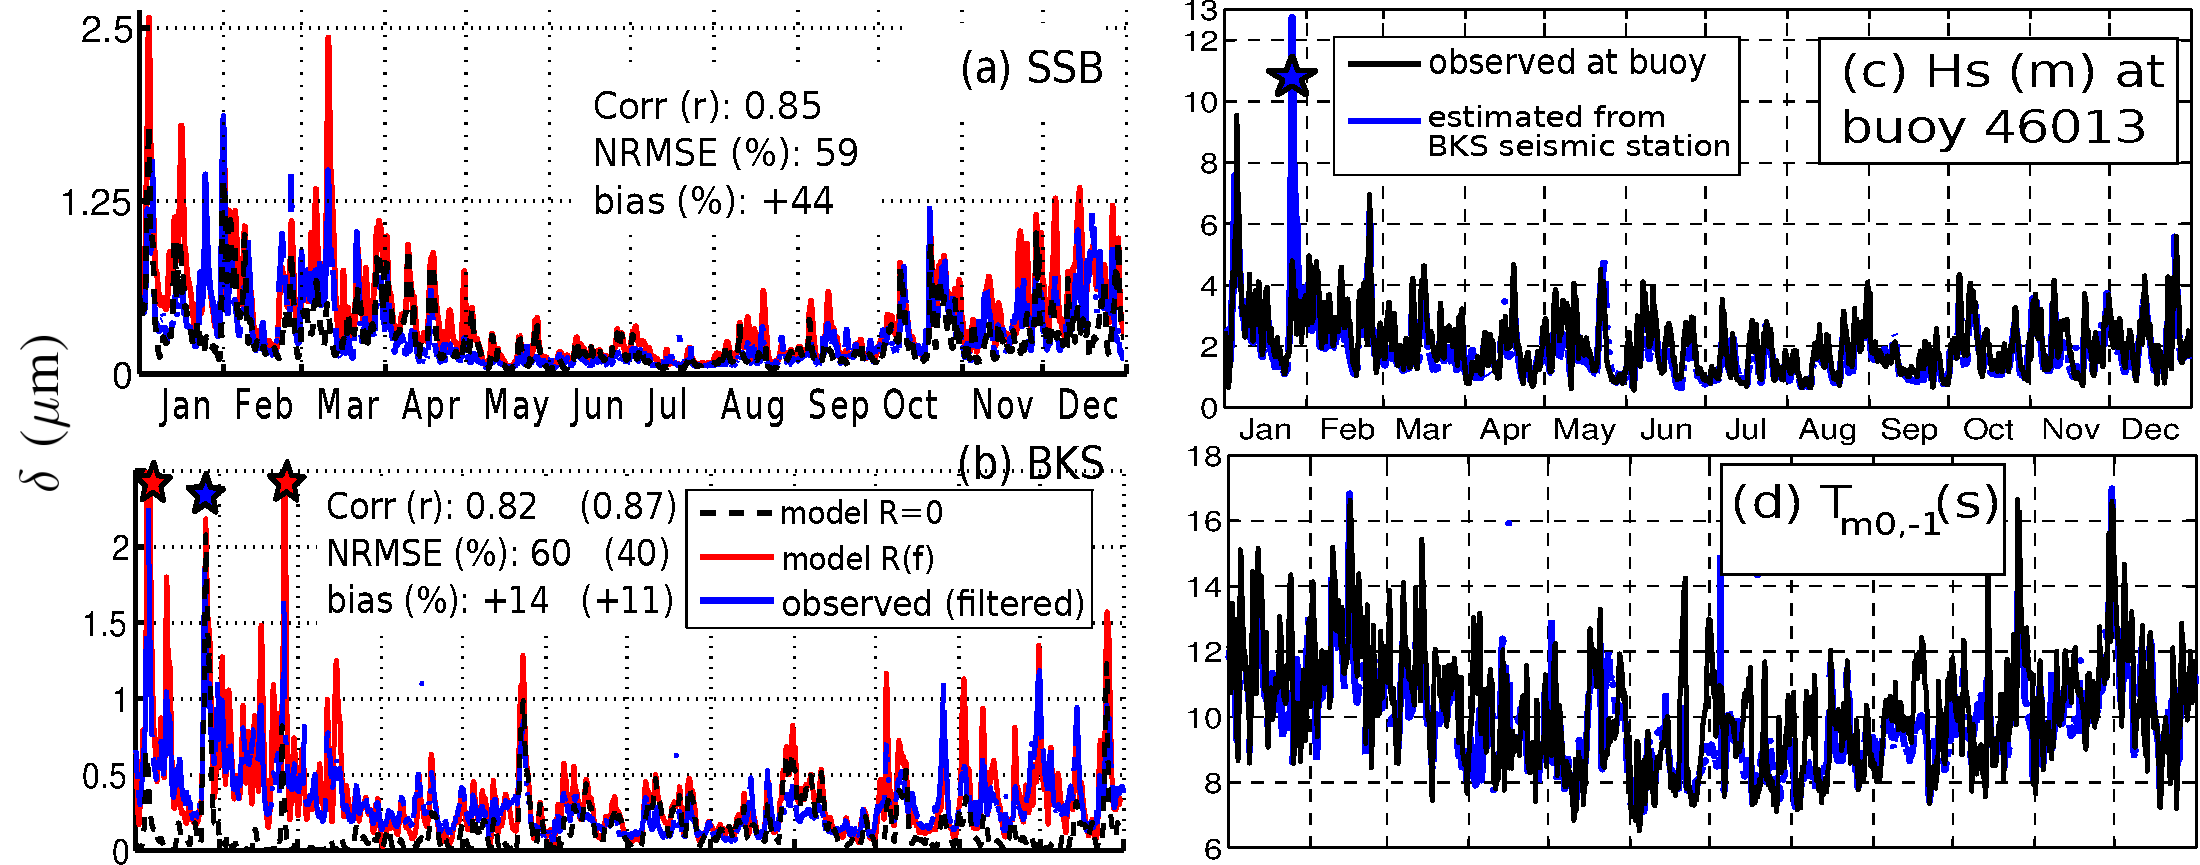
\includegraphics[width=\textwidth]{FIGS_CH_SISMO/timeseries_2008_BKS_SSB_only.pdf}}
%\vspace{3.64in}
  \caption{Relation entre signal sismique et houle coastal.}{Series temporelles du deplacement sismique vertical $\delta_{\mathrm{rms}}$
observe et modelise par l'equation (\ref{F_delta}) pour les stations (a) SSB et (b) BKS. 
(c) et (d) En bas, serie temporelle de hauteurs significatives et periode moyenne des vagues mesurees to 46013 et reconstruite to partir du signal sismique to BKS. 
}
\label{fig:sismo_timeseries}
\end{figure}
%%%%%%%%%%%%%%%%%%%%%%%%%%%%%%%%%%%%%%%%%%%%%%%%%%%%%%%%%%%%%%%%%%%%%%%%%%%%%

%\section{Measuring waves from microseisms}
%Microseisms are now widely used to for tomographic analysis 
%of the solid Earth structure \citep{Shapiro&al.2005}, and the monitoring of solid Earth properties. 
%Microseisms can also be used to estimate ocean wave properties. Cette application 
%fut envisagee des les annees 1930 et son utilisation pratique fut mise en oeuvre sur dans les annees 1970 sur la 
%coast ouest des Etats-Unis \citep{Zopf&al.1976}. A cette epoque la technologie de mesure par des bouees en mer n'etait pas 
%encore au point et il n'y avait pas d'autre moyen de mesure fiable. 

%Cette possibilite d'inverser le signal 
%sismique pour en deduire le spectre des vagues n'est toutefois pas universelle et certains types d'etat de mer peuvent causer 
%d'importantes erreurs. En effet, la relation d'inversion to partir du bruit  est typiquement bien calibree pour les 
%situations dans lesquelles la reflexion to la coast est la source principale du bruit. Or une houle opposee to une 
%mer du vent, ou deux houles se faisant face, peuvent aussi generer un tres fort bruit \citep{Obrebski&al.2012}.
%Dans ce cas la hauteur des vagues pourra be fortement surestimee. 
%Cette source d'erreur dejto discutee par \cite{Zopf&al.1976} est mise en evidence sur la figure \ref{fig:sismo_timeseries}.c 
%pour l'estimation des vagues to partir de la station BKS. Ainsi, le 26 janvier 2008, une situation meteorologique particuliere 
%produit un fort bruit dont on deduit une hauteur significative qui depasse 12~m, soit plus que la hauteur centennale, 
%alors que en realite, la hauteur des vagues n'a pas depasse 5.5~m ce jour lto dans la sone coastal (figure \ref{fig:BKS_odd_case}). 

%%%%%%%%%%%%%%%%%%%%%%%%%%%%%%%%%%%%%%%%%%%%%%%%%%%%%%%%%%%%%%%%%%%%%%%%%%%%%
%\begin{figure}
%\centerline{\includegraphics[width=0.8\textwidth]{FIGS_CH_SISMO/BKS_january_2008_case_v5.pdf}}
% \caption{Map of the wave-induced second order surface pressure variance, integrated across frequencies  (couleurs), on  26 January 2008 at 12:00 UTC, off the  California coast. Cette situation correspond to de une forte houle du nord-ouest et une depression (L) centree en 32$^\circ$ N  132$^\circ$ W.  Les parametres d'etat de mer sont symbolises pour trois positions  (carres), avec la mer du vent (groups of three arrows, and heights $H_{s0}$),  et les houles quand elles existent (dotted arrows and heights $H_{s1}$ and  $H_{s2}$). La depression produit des vents depassant les 25 m/s, ce qui, to l'ouest amplifiela houle incidente en mer forte  ($H_s$ jusqu'to 8~m). A l'est de la depression, des mers agitees  (4~m) se transforment en houle au nord du front atmospherique  (ligne avec triangles).  Tous ces champs de vauges produisent deux maxima de pression qui generent des microseismes. Le plus fort  (2600~hPa$^2$m$^2$)  s'etend le long du front froid autour du point $A$, il est cause par la mer du vent qui s'oppose to la houle de  nord-ouest.   Le second maximum, au point $B$, vient de l'interaction des deux houles.  Enfin on notr que en  $C$, les pressions induites par les vagues sont faibles  (200~hPa$^2$m$^2$) car il n'y a pas de houle opposee to la mer du vent qui pourrait donner une forte valeur de $I(f)$ (eq. \ref{eq:I}). Si $I(f)$ en $C$ etait aussi fort qu'en $A$, alors la source microsismique y serait 200 fois plus forte.} \label{fig:BKS_odd_case} 
%\end{figure}
%%%%%%%%%%%%%%%%%%%%%%%%%%%%%%%%%%%%%%%%%%%%%%%%%%%%%%%%%%%%%%%%%%%%%%%%%%%%%

%Il convient donc d'ameliorer sensiblement la methode pour arriver to une estimation robuste des parametres d'etat de mer 
%to partir du bruit sismique. Dans le cas de stations sismiques sensibles to une vaste zone de l'ocean l'interpretation quantitative 
%du signal n'est pas simple mais il y a une correlation entre la hauteur des vagues sur l'ensemble de l'Atlantique nord-est et 
%l'intensite du bruit sismique en Europe de l'ouest. Une modelisation numerique des vagues et du bruit peut 
%permettre de filtrer les evenements anormaux \citep{Ardhuin&al.2012}. 


